





%----------------------------------------------------------------------------------------

\newpage

%%%%%%%%%%%%%%%%%%%%%%%
\section{Exploration of the SimpopNet model}{Exploration du modèle SimpopNet}

\label{app:sec:macrocoevolexplo}




%%%%%%%%%%%%%%%%%
%\begin{figure}
    %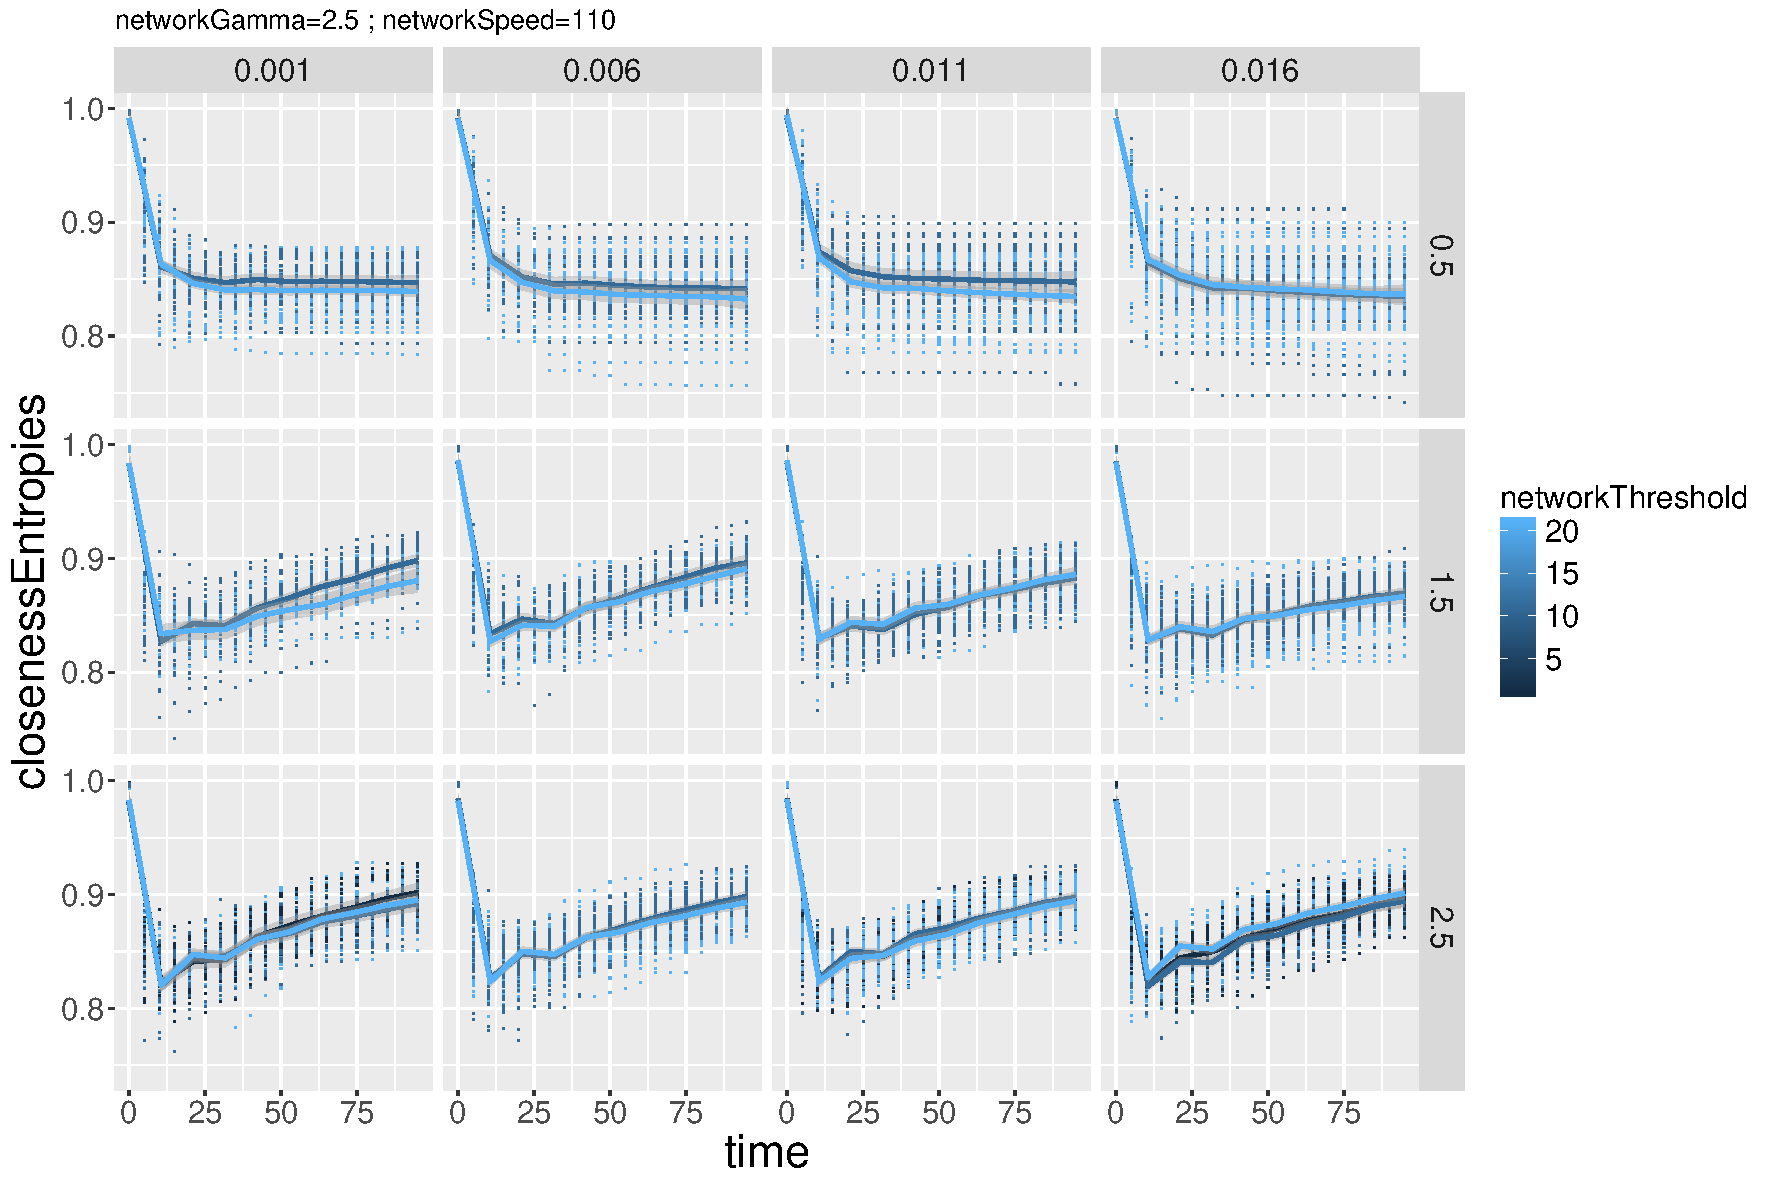
\includegraphics[width=0.48\linewidth]{Figures/MacroCoEvolExplo/closenessEntropies_networkGamma2_5_networkSpeed110}
	%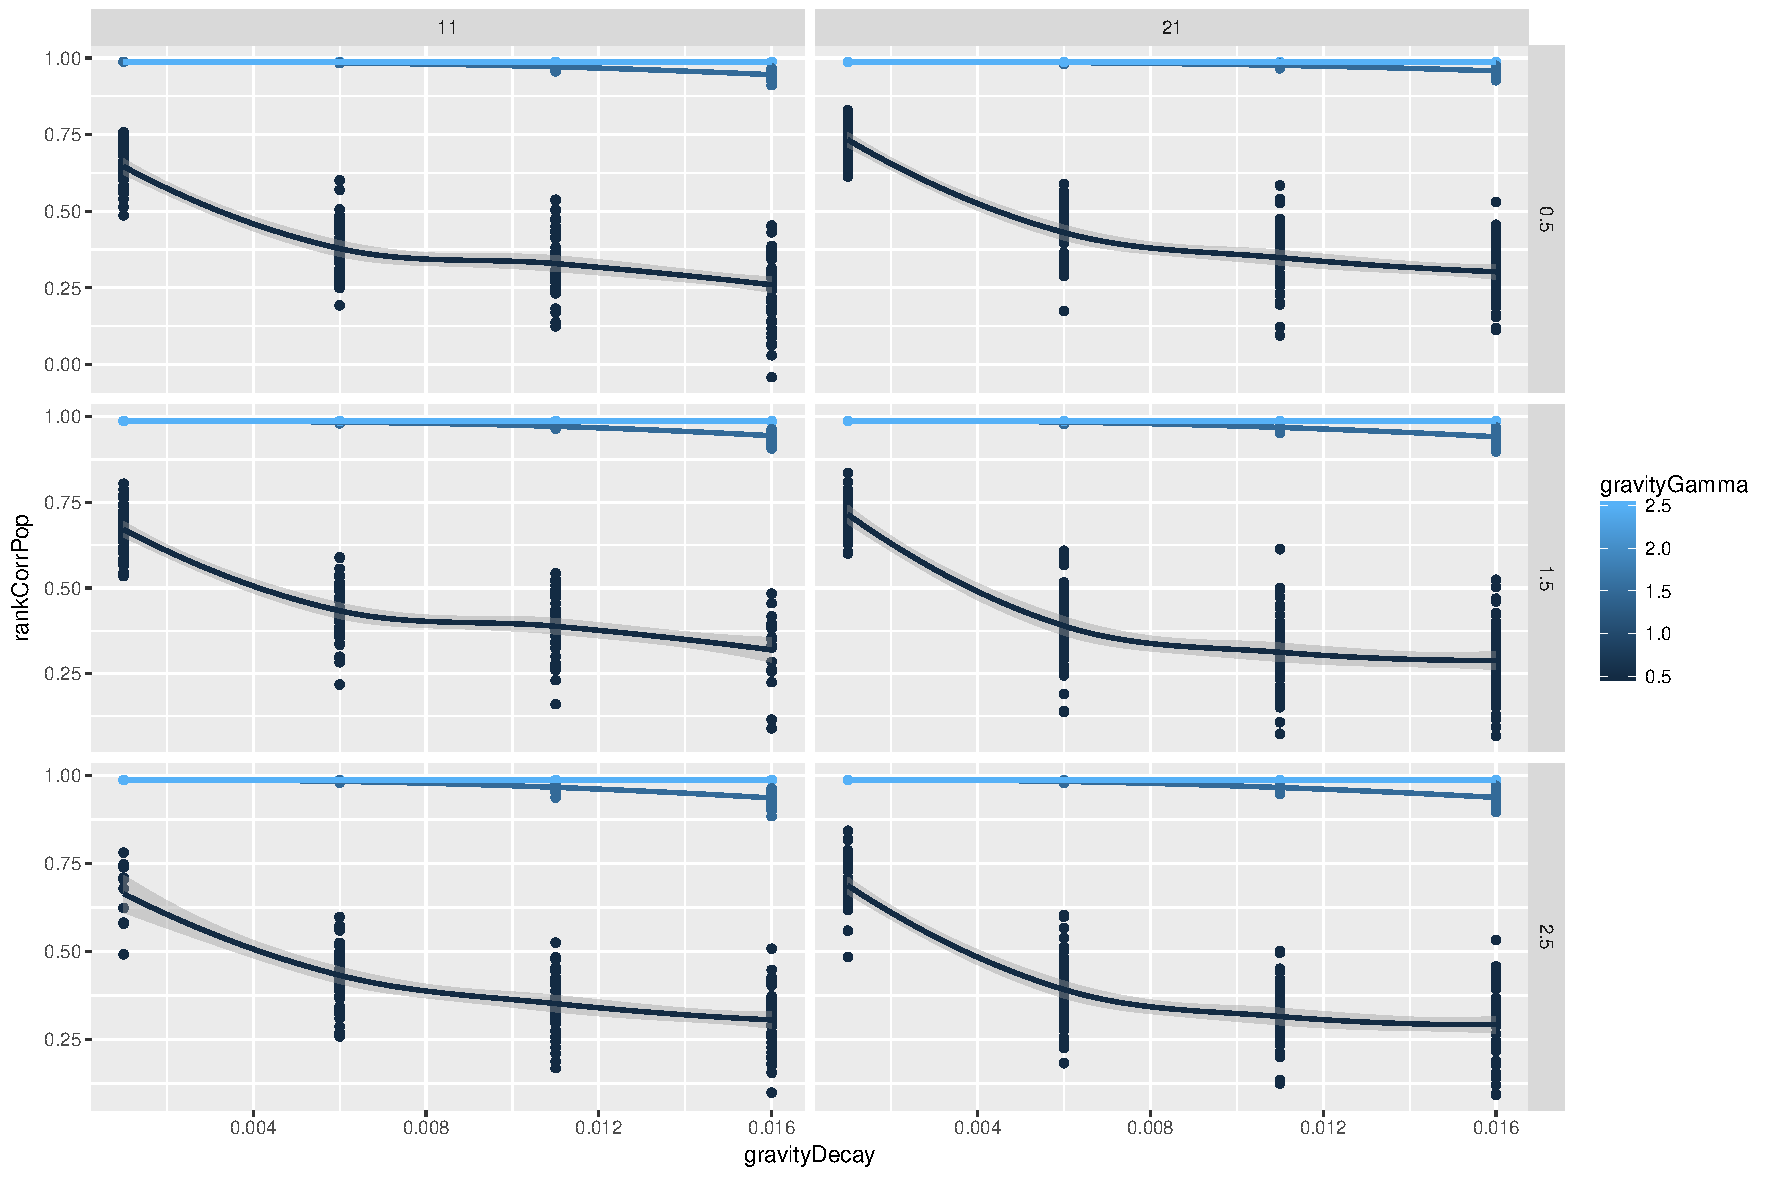
\includegraphics[width=0.48\linewidth]{Figures/MacroCoEvolExplo/rankCorrPop_synthRankSize0_5_networkSpeed10}
%\appcaption{}{}
%\end{figure}
%%%%%%%%%%%%%%%%%




%%%%%%%%%%%%%%%%%
%\begin{figure}
%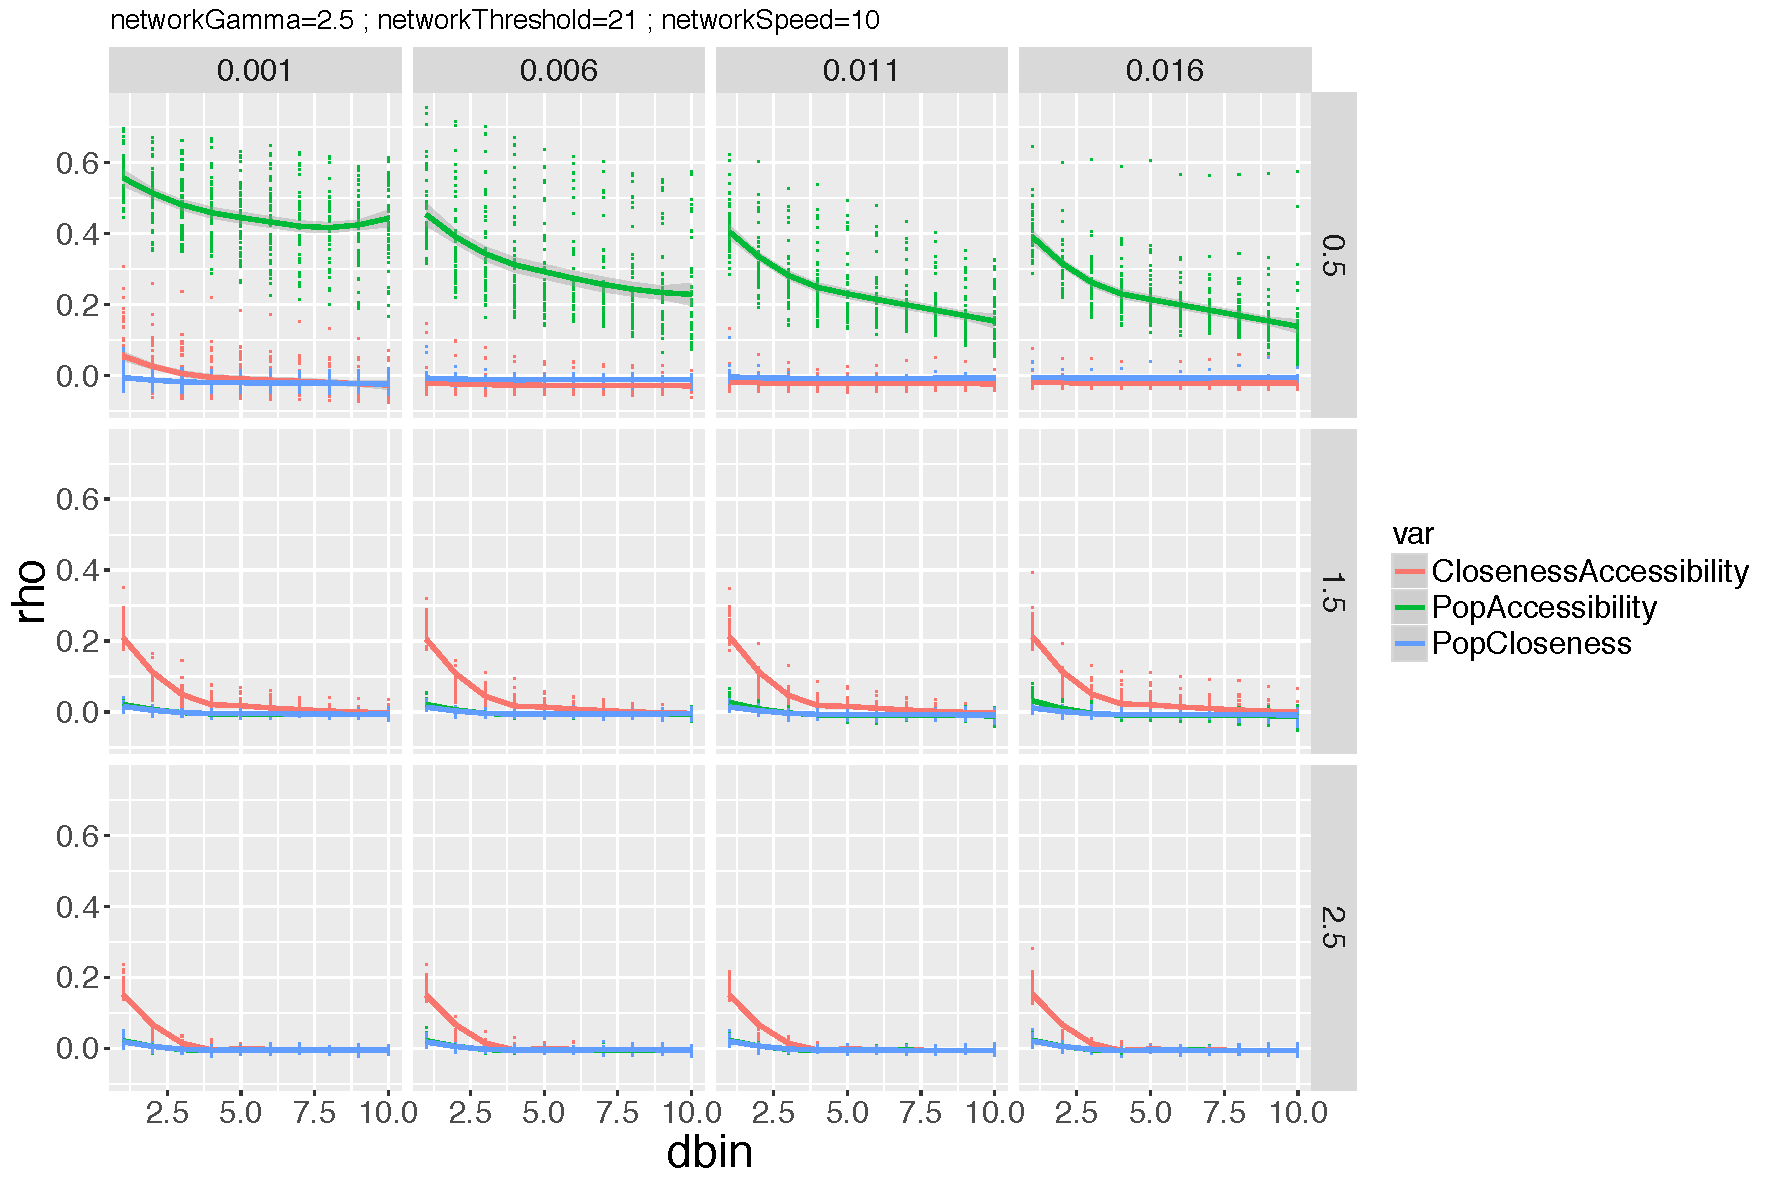
\includegraphics[width=0.48\linewidth]{Figures/MacroCoEvolExplo/distcorrs_networkGamma2_5_networkThreshold21_networkSpeed10}
	%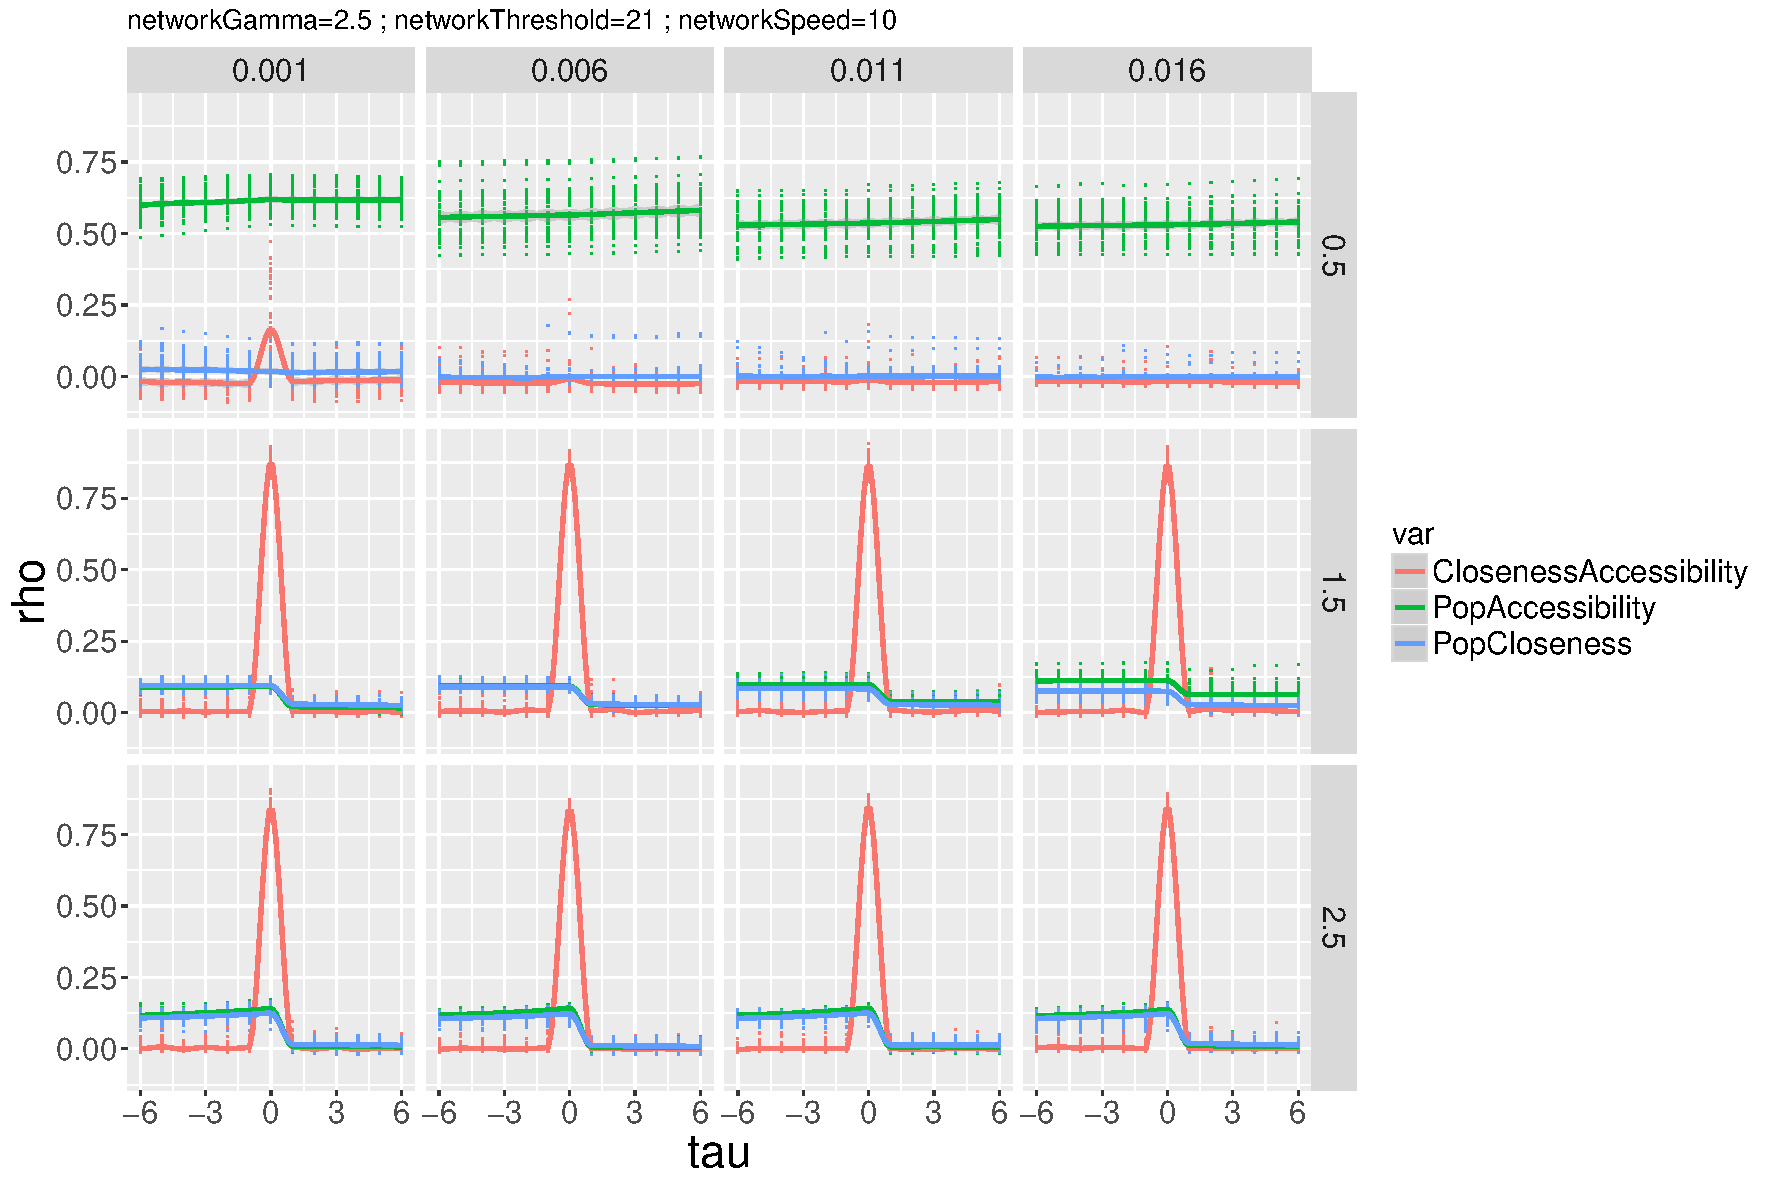
\includegraphics[width=0.48\linewidth]{Figures/MacroCoEvolExplo/laggedcorrs_networkGamma2_5_networkThreshold21_networkSpeed10}
%\appcaption{}{}
%\end{figure}
%%%%%%%%%%%%%%%%%








%----------------------------------------------------------------------------------------

\newpage

%%%%%%%%%%%%%%%%%%%%%%%
\section{Macroscopic co-evolution model}{Modèle de co-évolution macroscopique}

\label{app:sec:macrocoevol}



%%%%%%%%%%%%%%%%%%%
\subsection{Synthetic data}{Données synthétiques}



%%%%%%%%%%%%%
\begin{figure}
%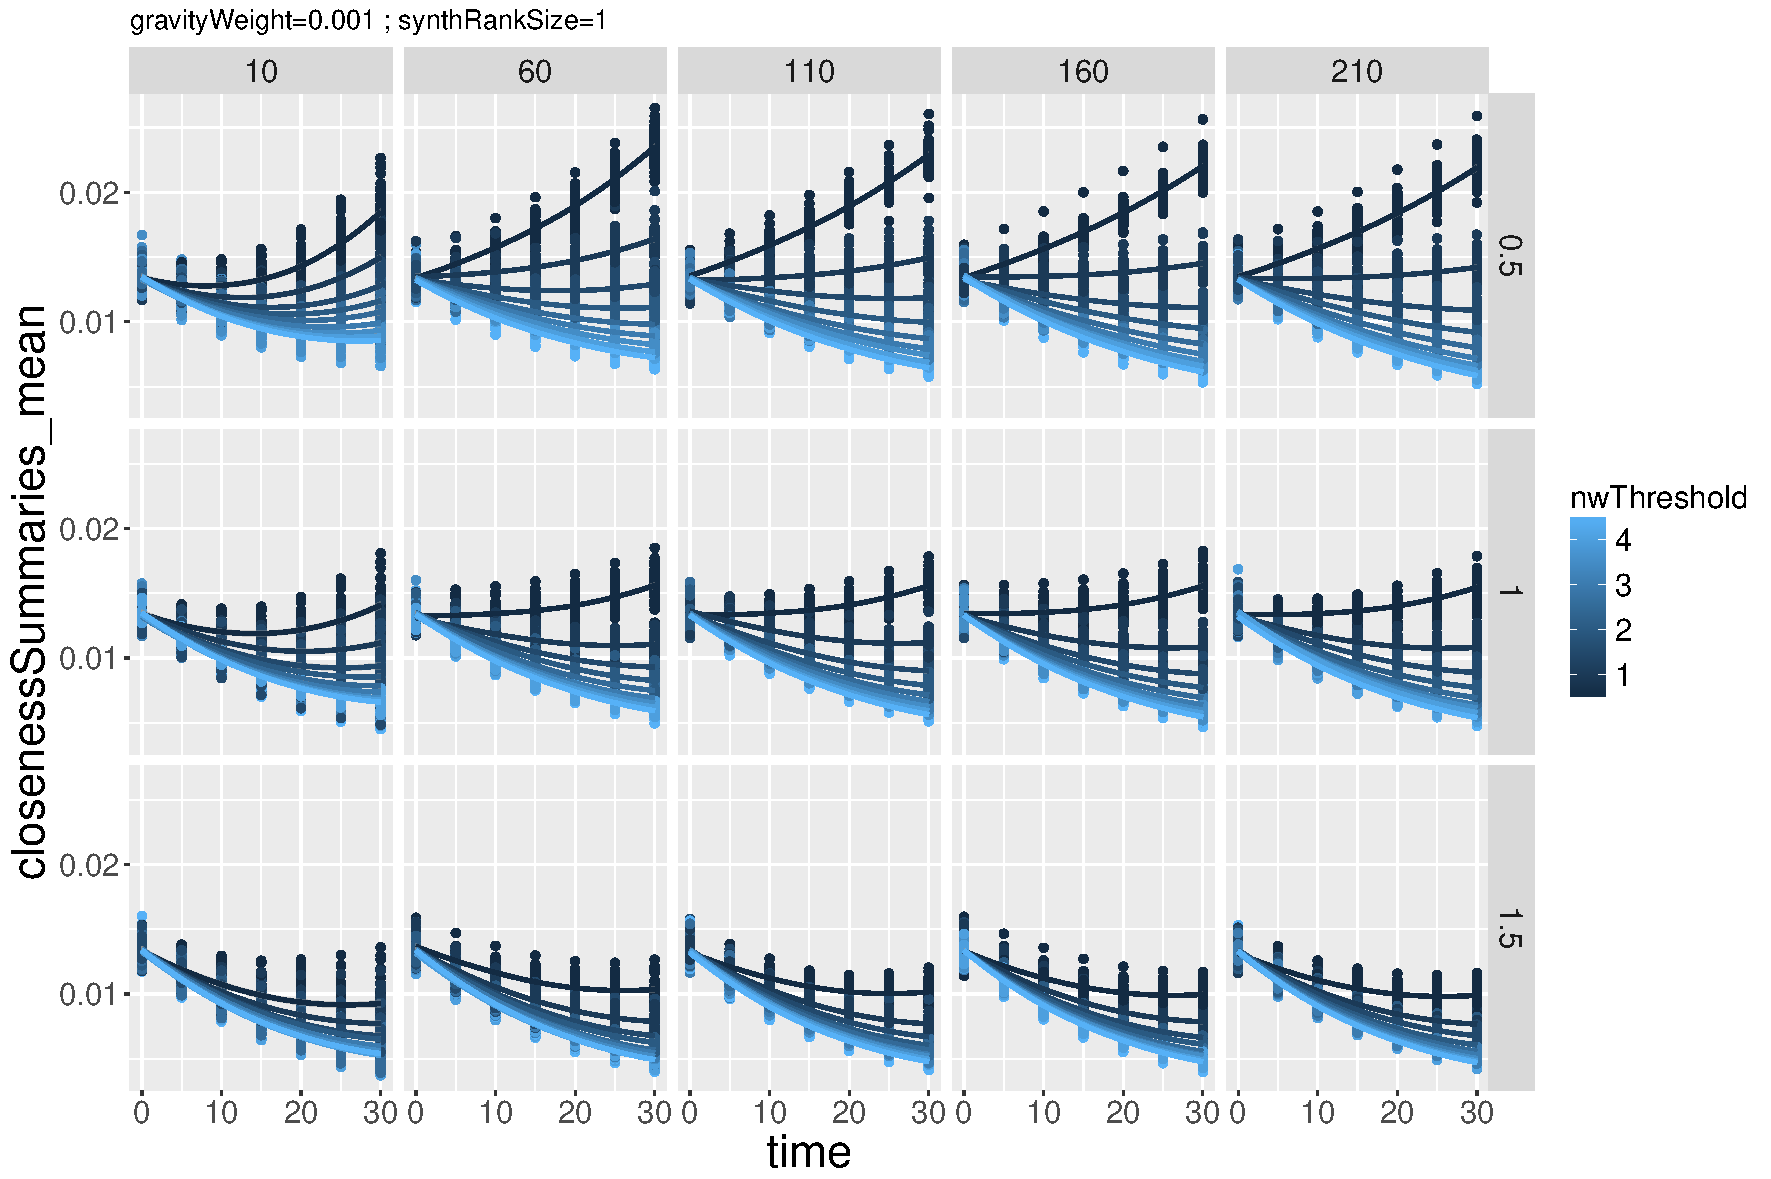
\includegraphics[width=0.48\linewidth]{Figures/MacroCoEvol/closenessSummaries_meansynthRankSize1_gravityWeight0_001.pdf}
%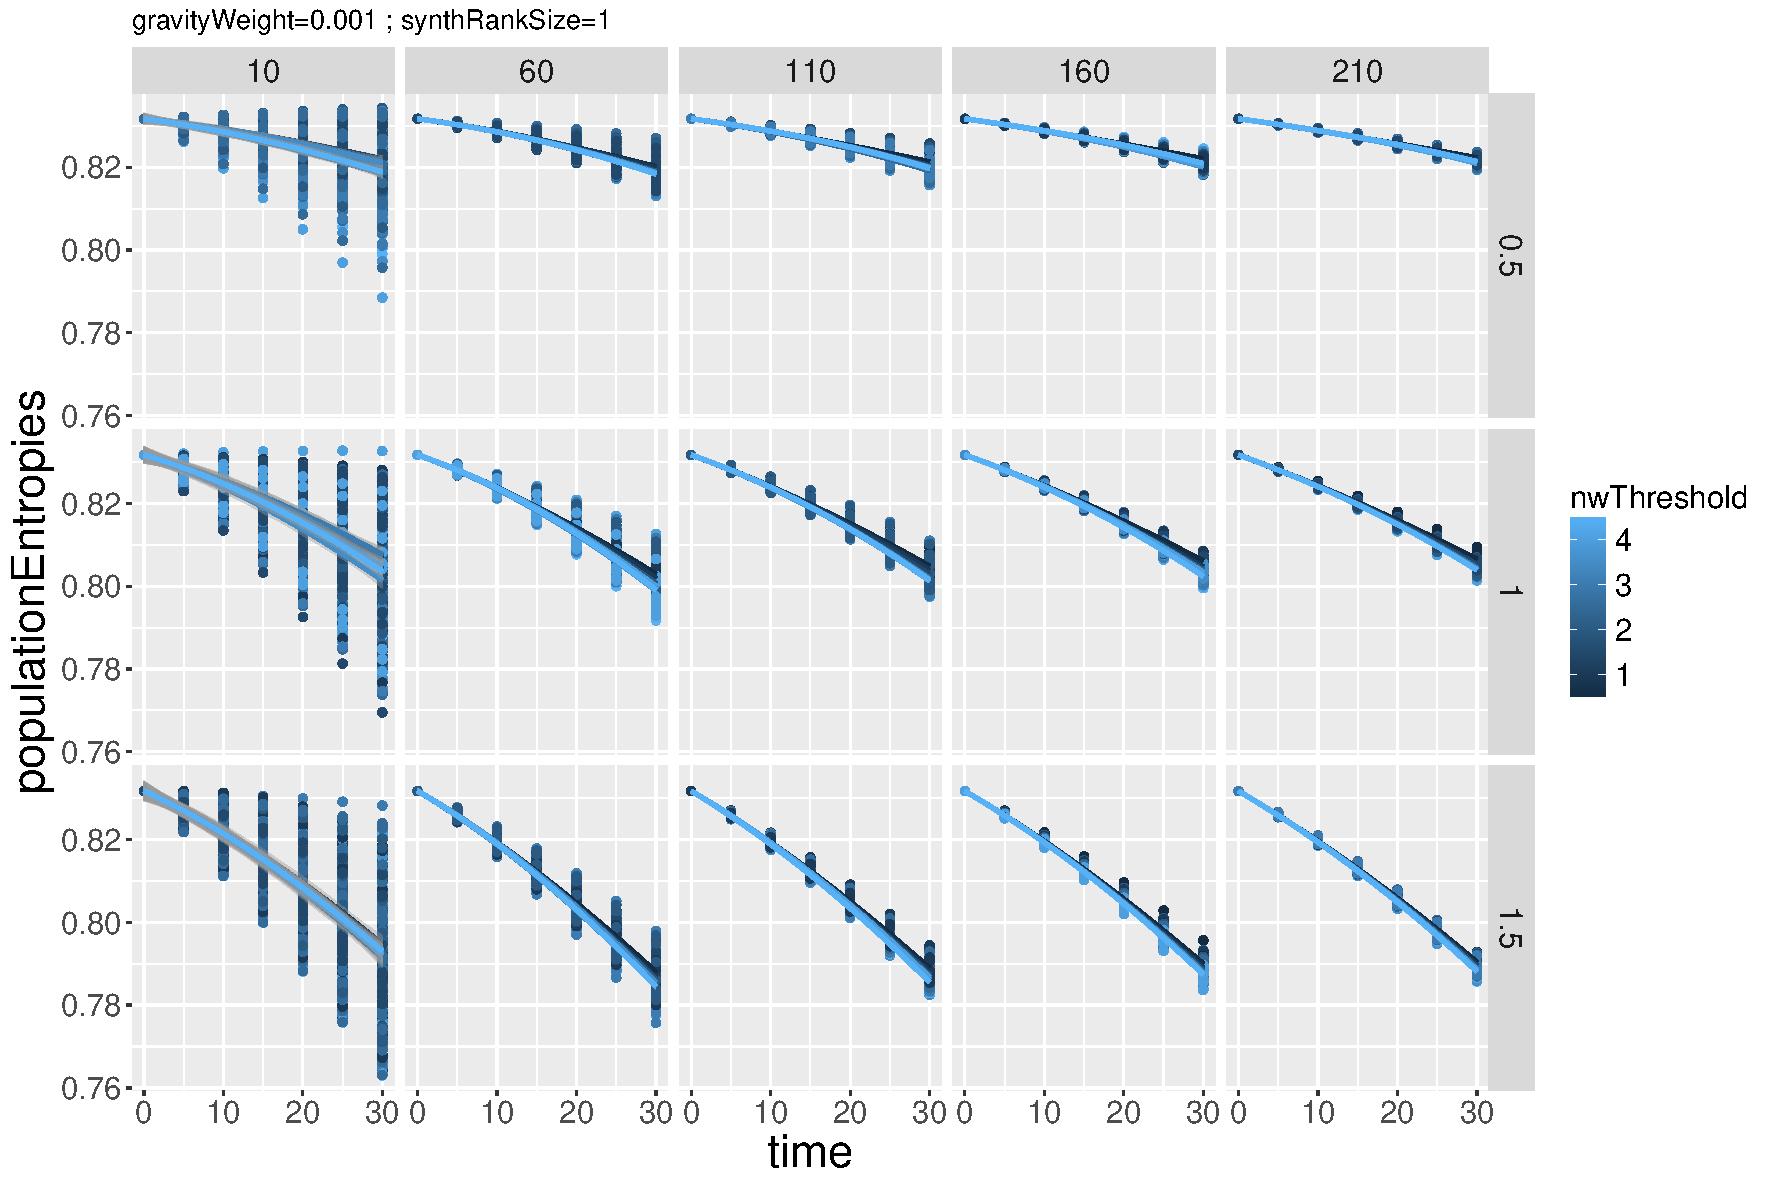
\includegraphics[width=0.48\linewidth]{Figures/MacroCoEvol/populationEntropiessynthRankSize1_gravityWeight0_001.pdf}
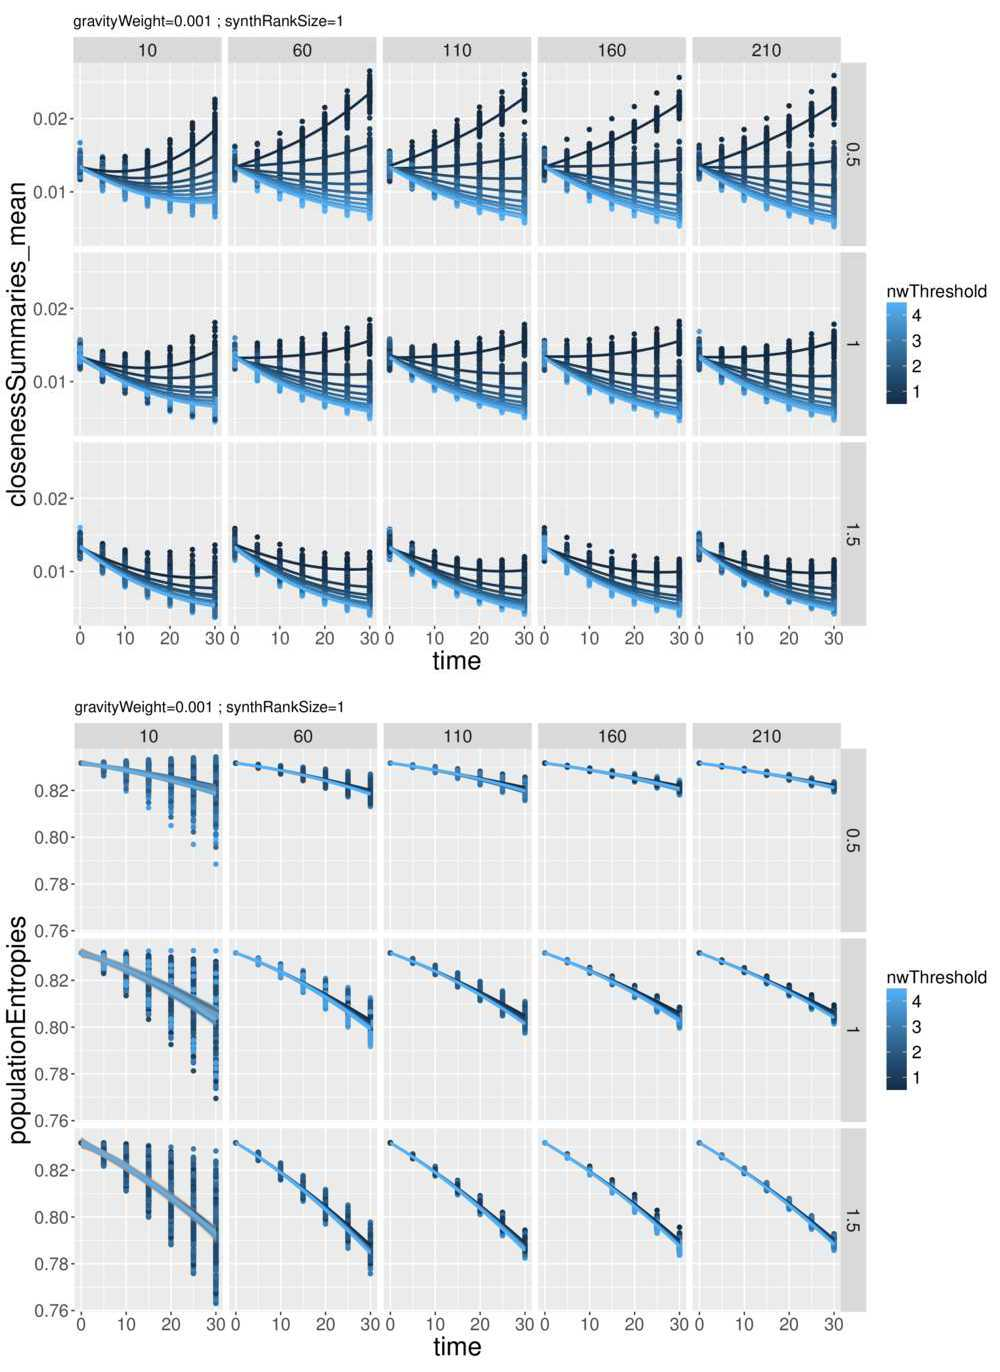
\includegraphics[width=\linewidth,height=0.9\textheight]{Figures/Final/A-macrocoevol-behavior-time.jpg}
\appcaption{\textbf{Behavior of the co-evolution model.}\label{fig:macrocoevol:behavior-time}}{\textbf{Comportement du modèle de co-evolution avec réseau abstrait sur un système de villes synthétique, pour $\alpha_S = 1$.} \textit{(Haut)} Moyenne des centralités de proximité, en fonction du temps, pour $d_G$ (colonnes), $\gamma_G$ (lignes) et $\phi_0$(couleur) variables, à $w_G = 0.001$ fixé ; \textit{(Bas)} Entropie de populations, en fonction du temps, pour $d_G$ (colonnes), $\gamma_G$ (lignes) et $\phi_0$(couleur) variables, à $w_G = 0.001$ fixé Se référer au texte pour l'interprétation.\label{fig:app:macrocoevol:behavior-time}}
\end{figure}
%%%%%%%%%%%%%








%%%%%%%%%%%%%
\begin{figure}
%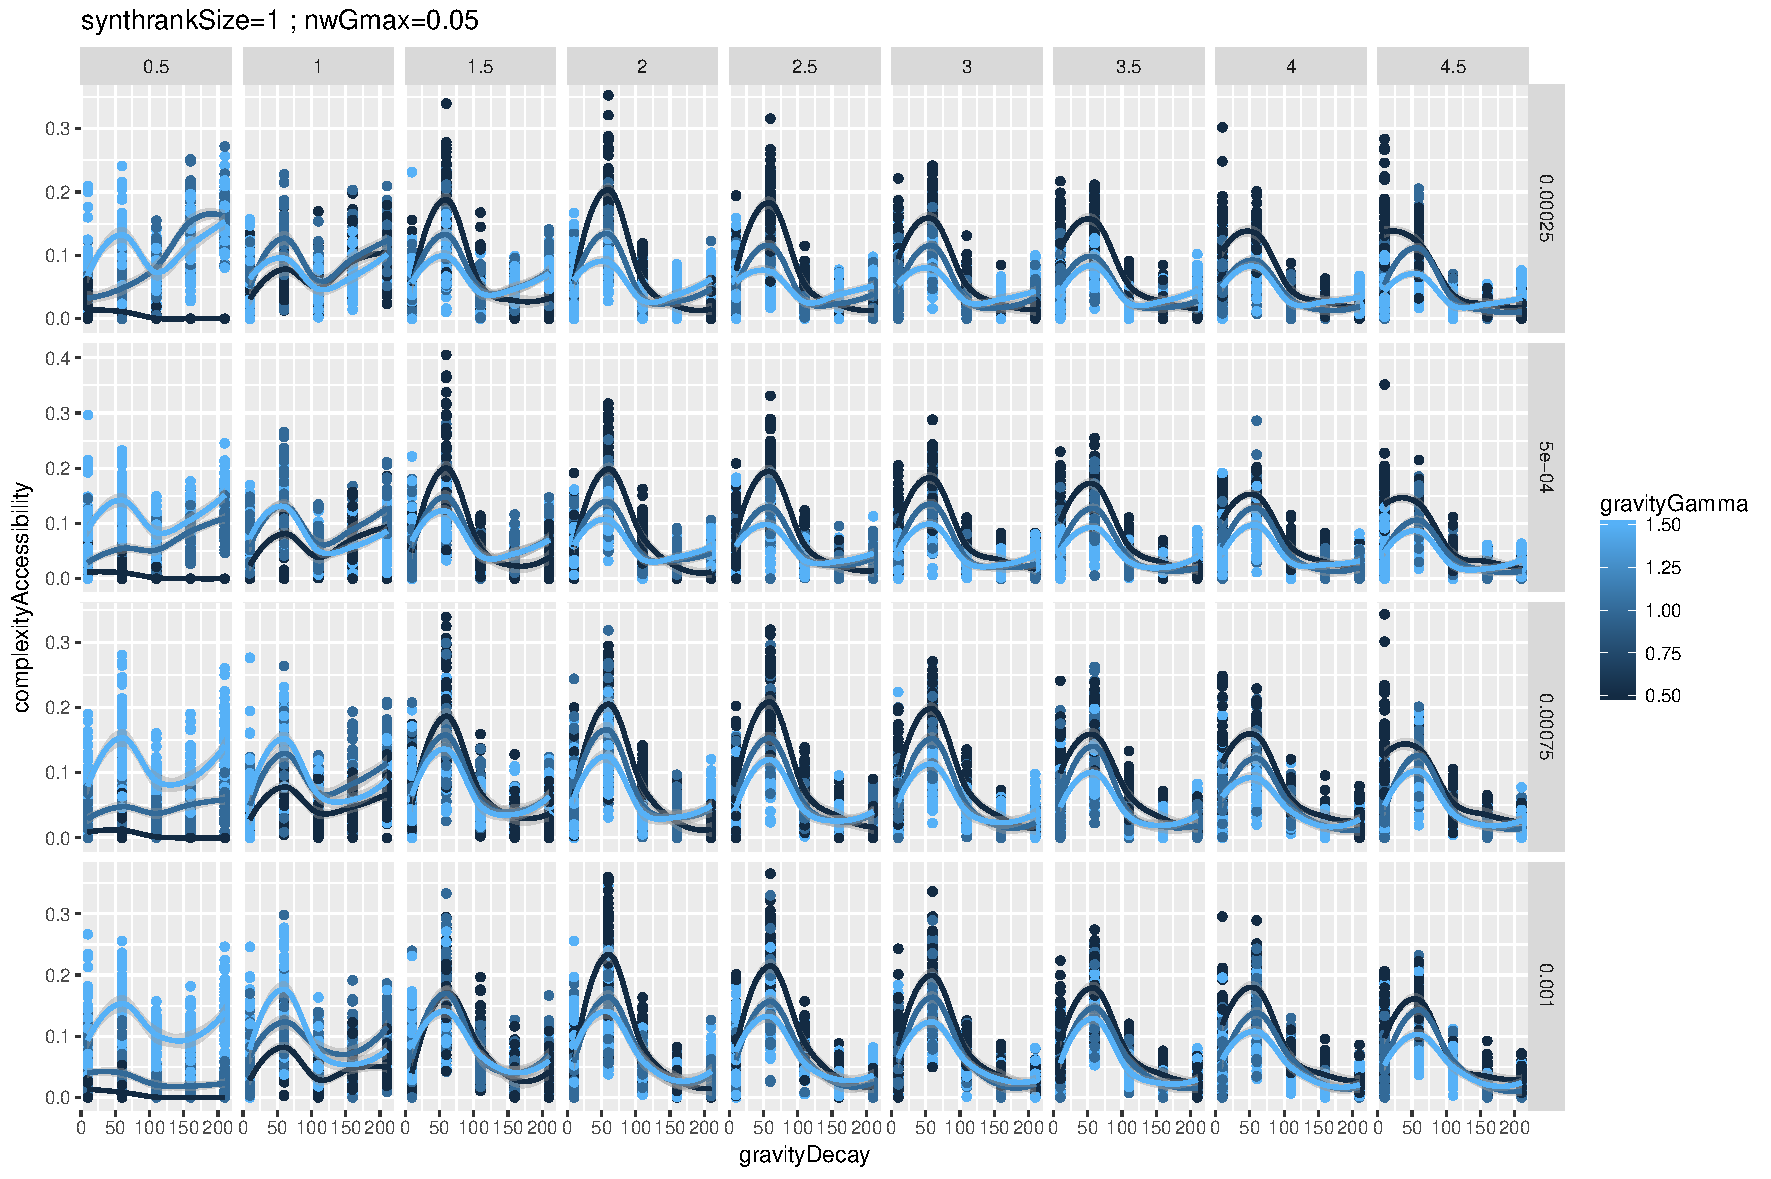
\includegraphics[width=0.48\linewidth]{Figures/MacroCoEvol/complexityAccessibility_synthrankSize1_nwGmax0_05}
%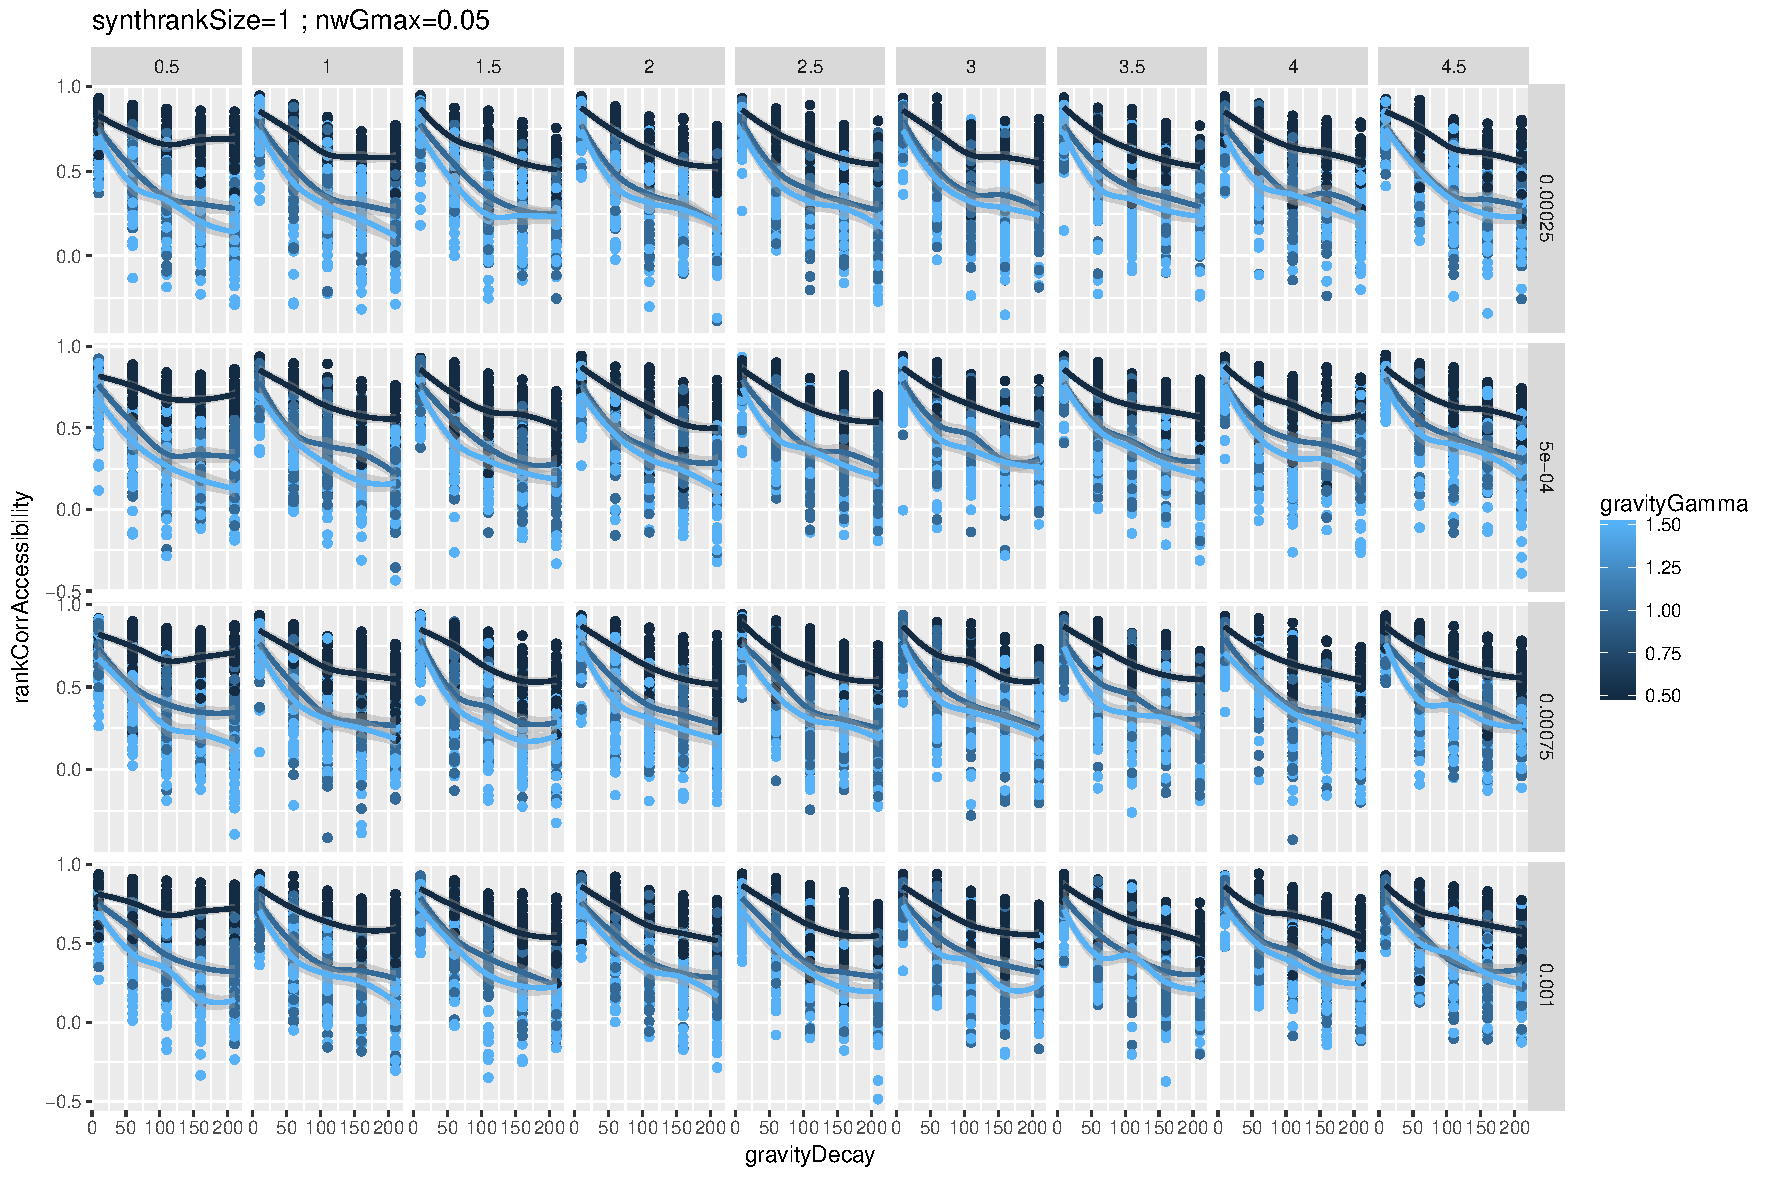
\includegraphics[width=0.48\linewidth]{Figures/MacroCoEvol/rankCorrAccessibility_synthrankSize1_nwGmax0_05}
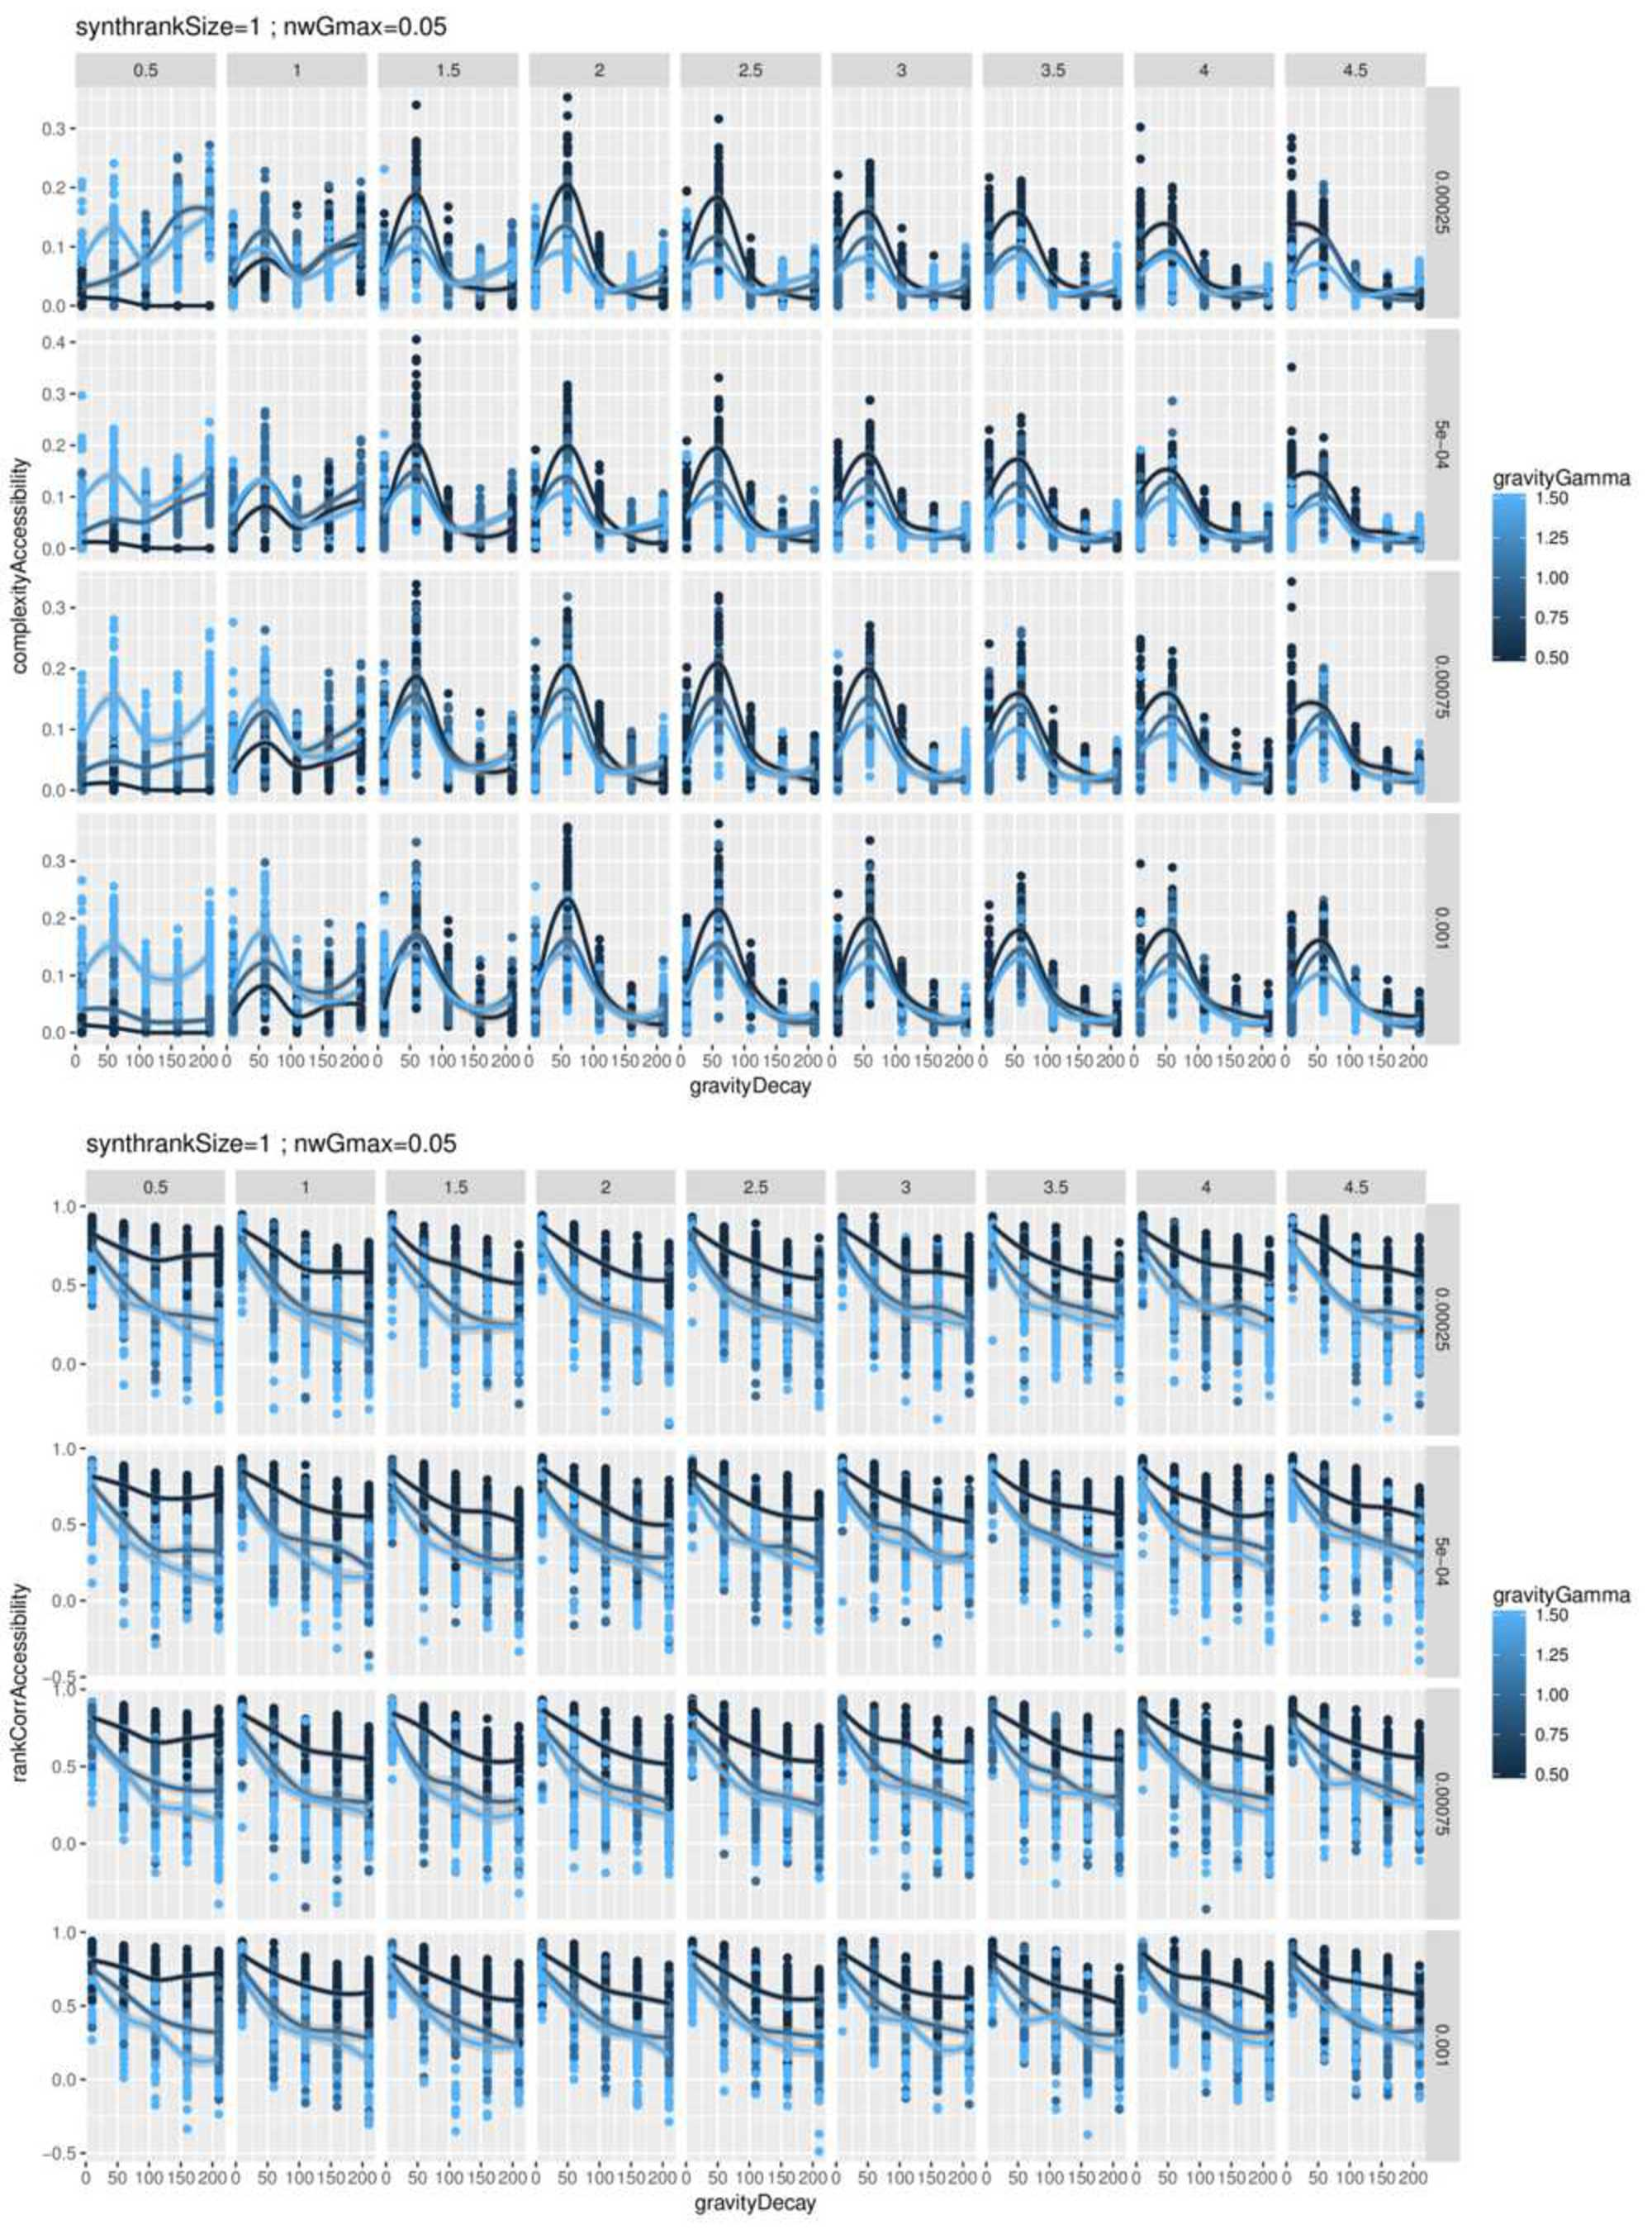
\includegraphics[width=\linewidth]{Figures/Final/A-macrocoevol-behavior-aggreg.jpg}
\appcaption{}{\textbf{} \textit{(Haut)} Complexité des accessibilités, en fonction de $d_G$, pour $\phi_0$ (colonnes), $w_G$ (lignes) et $\gamma_G$ (couleur) variables ; \textit{(Bas)} Corrélations de rang des accessibilités, pour les mêmes paramètres.\label{fig:app:macrocoevol:behavior-aggreg}}
\end{figure}
%%%%%%%%%%%%%





%%%%%%%%%%%%%
\begin{figure}
%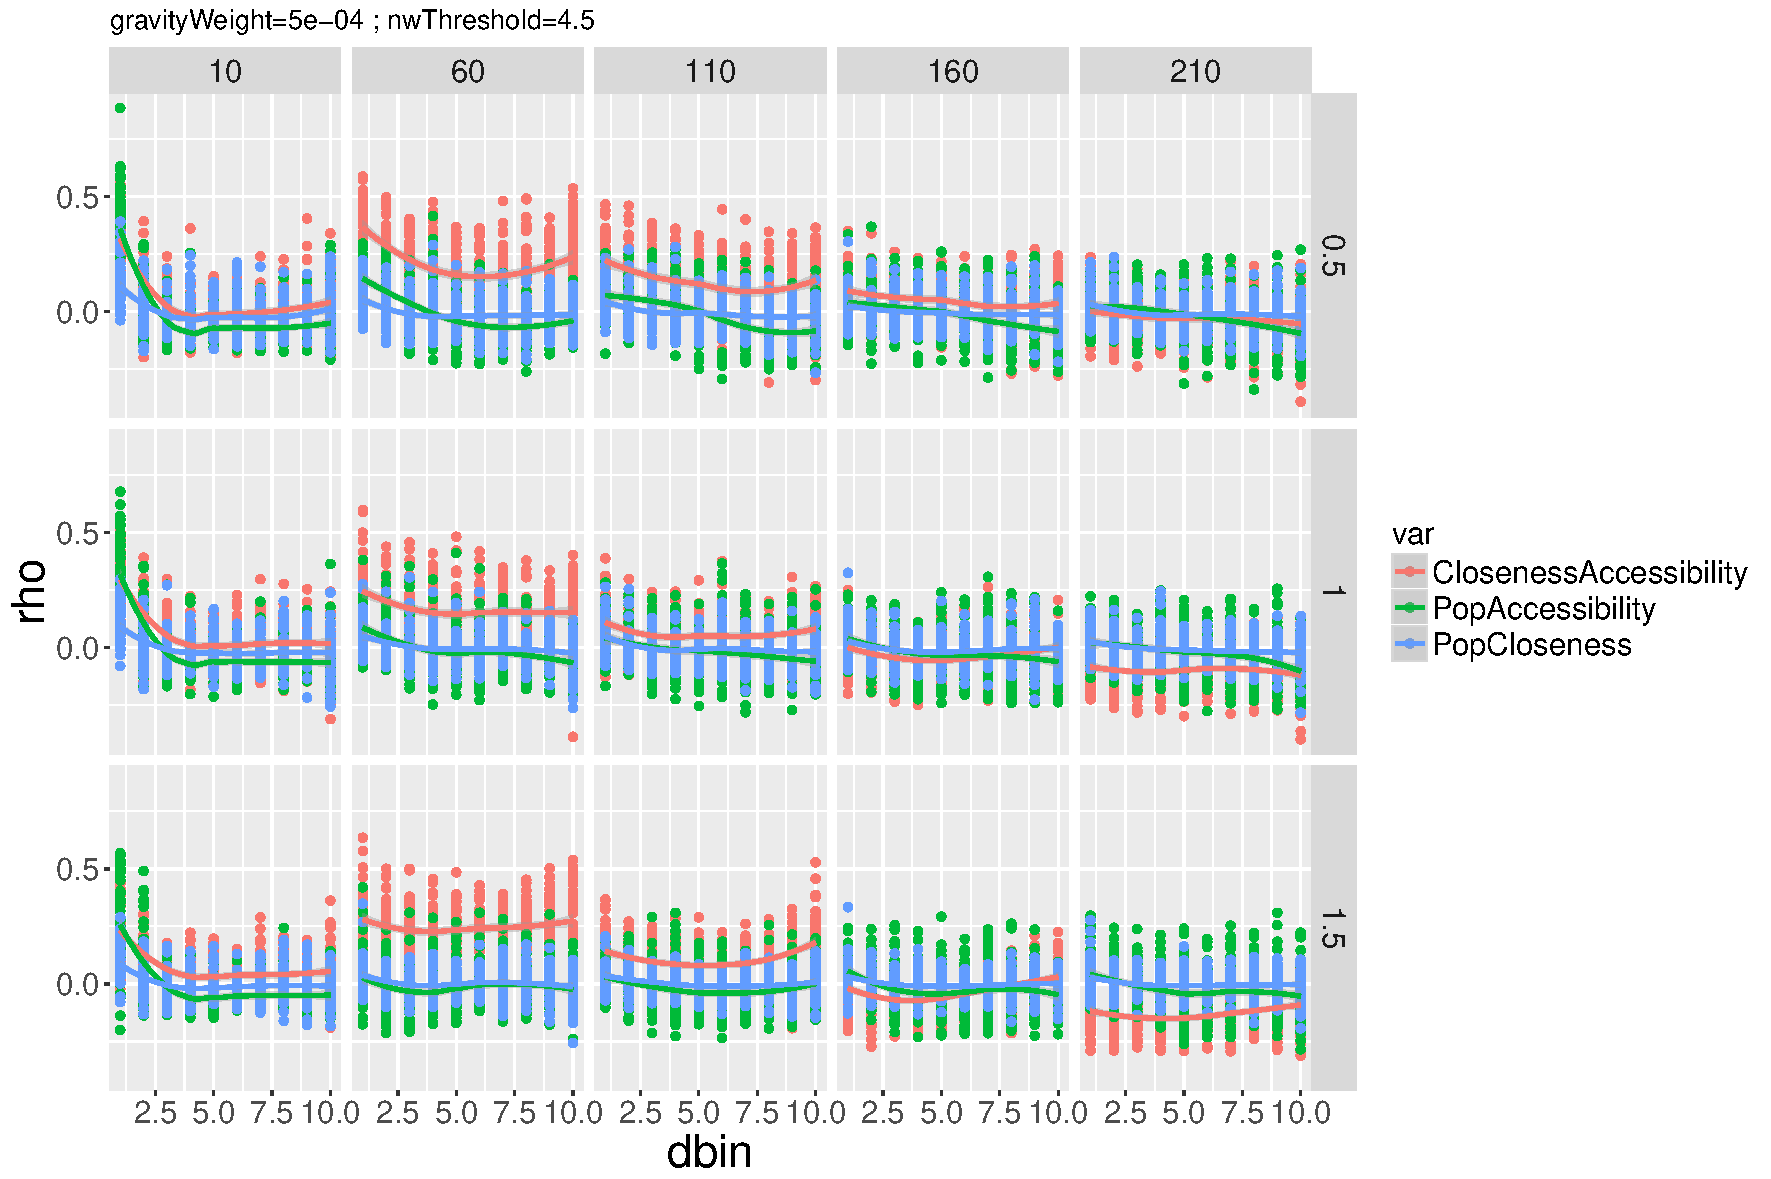
\includegraphics[width=0.9\linewidth]{Figures/MacroCoEvol/distcorrs_gravityWeight5e-04_nwThreshold4_5}
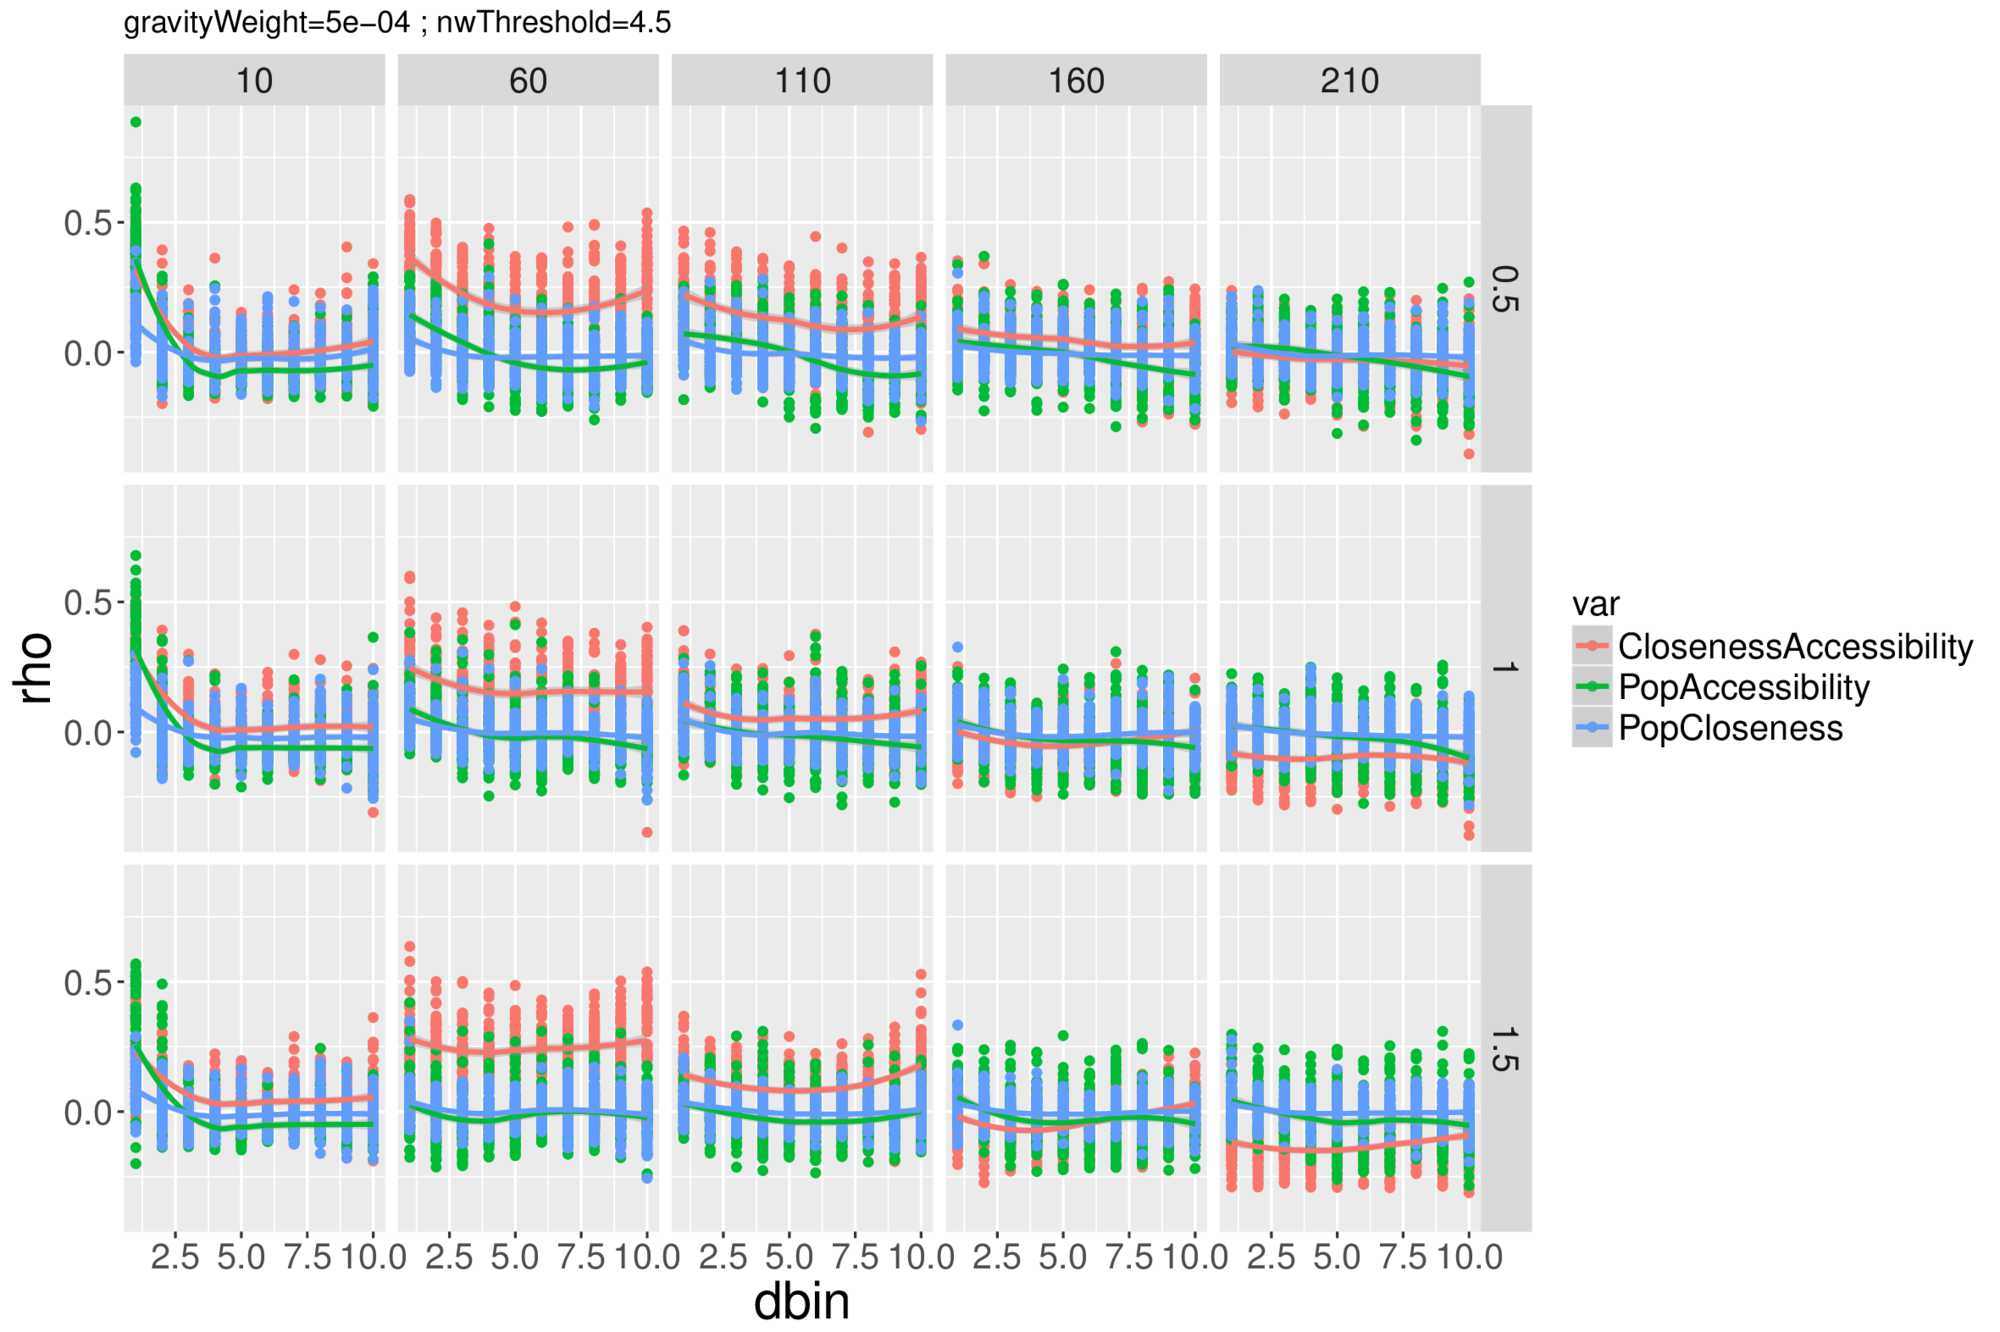
\includegraphics[width=\linewidth]{Figures/Final/A-macrocoevol-distcorrs.jpg}
\appcaption{\label{fig:app:macrocoevol:distcorrs}}{\textbf{Corrélations en fonction de la distance.} Correlation $\rho_d$ entre couples de variables (donné par la couleur), en fonction de la distance $d$ (discrétisée en déciles), pour $d_G$ variable (colonnes) et $\gamma_G$ variable (lignes), à $w_G = 5e-4$ et $\phi_0 = 4.5$
\label{fig:app:macrocoevol:distcorrs}}
\end{figure}
%%%%%%%%%%%%%


%%%%%%%%%%%%%
\begin{figure}
%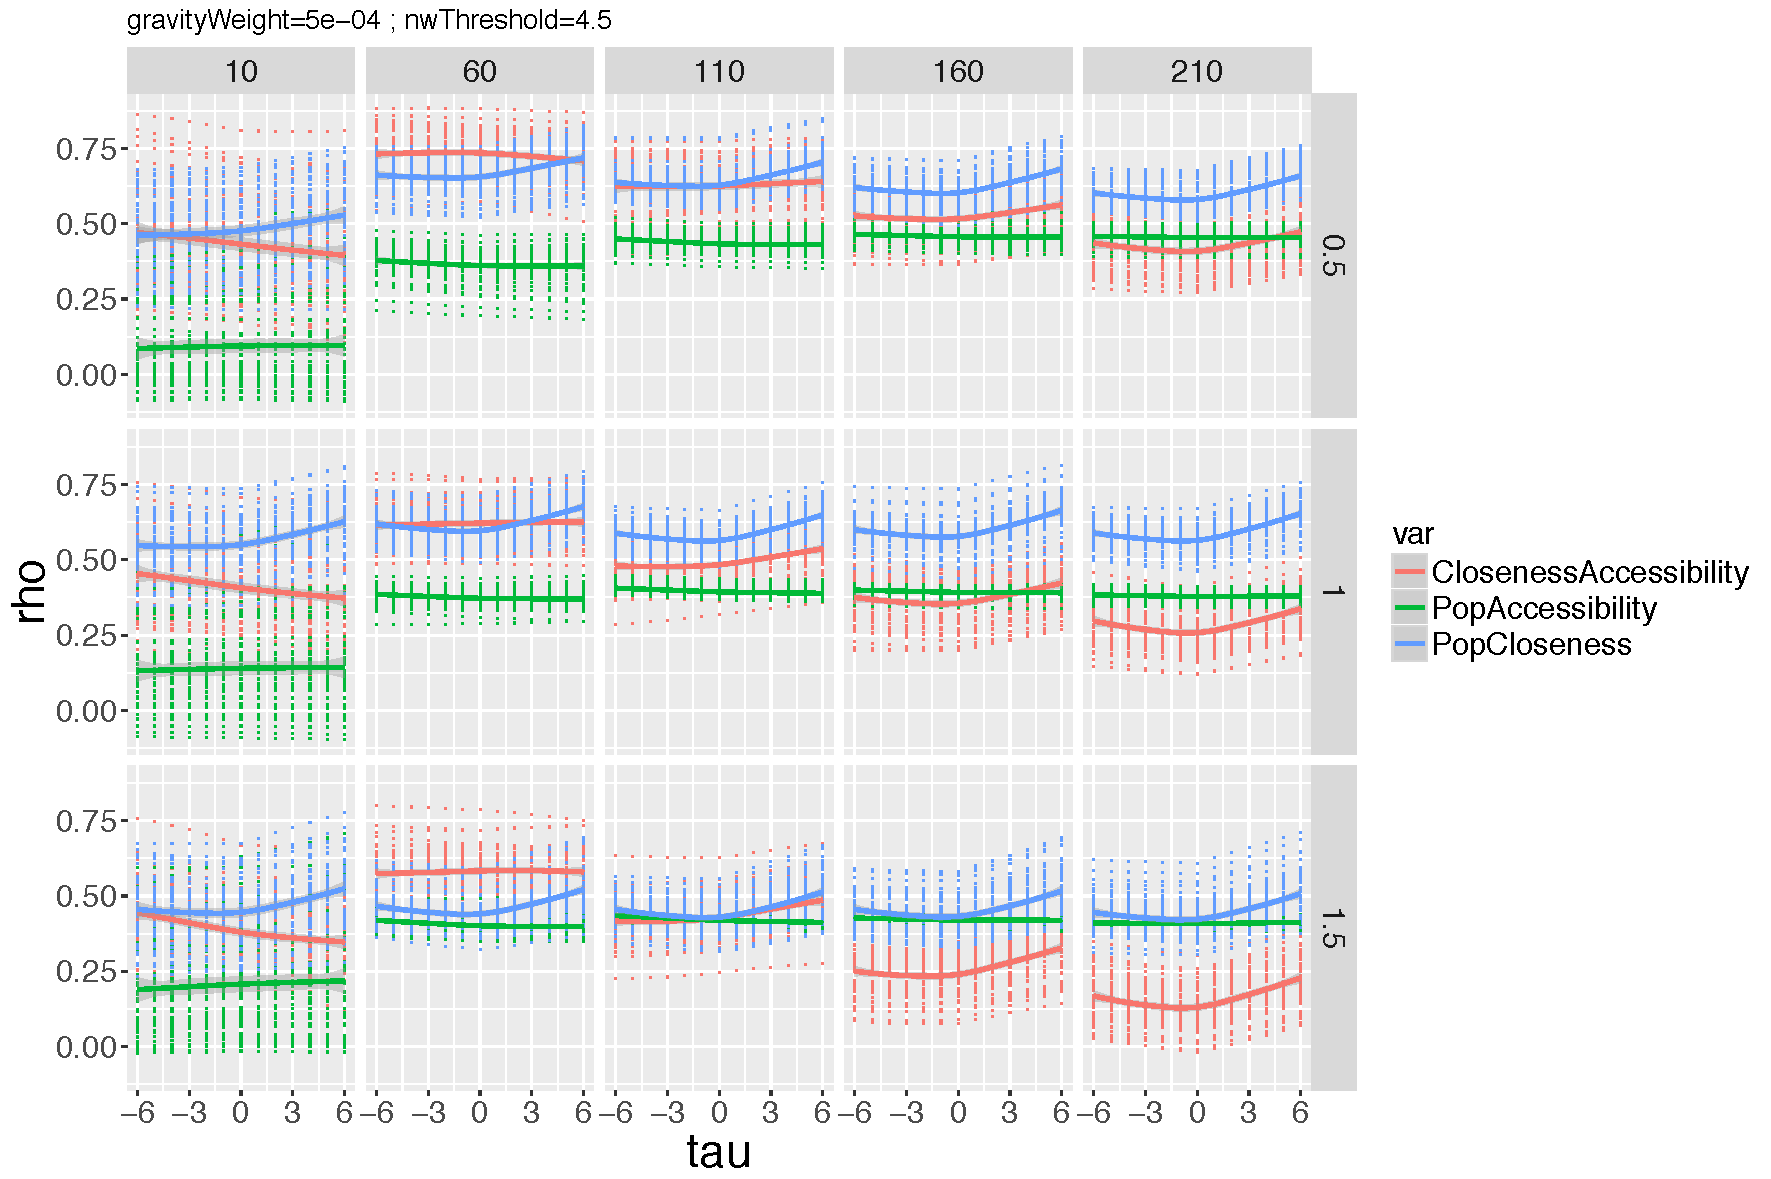
\includegraphics[width=0.9\linewidth]{Figures/MacroCoEvol/laggedcorrs_gravityWeight5e-04_nwThreshold4_5}
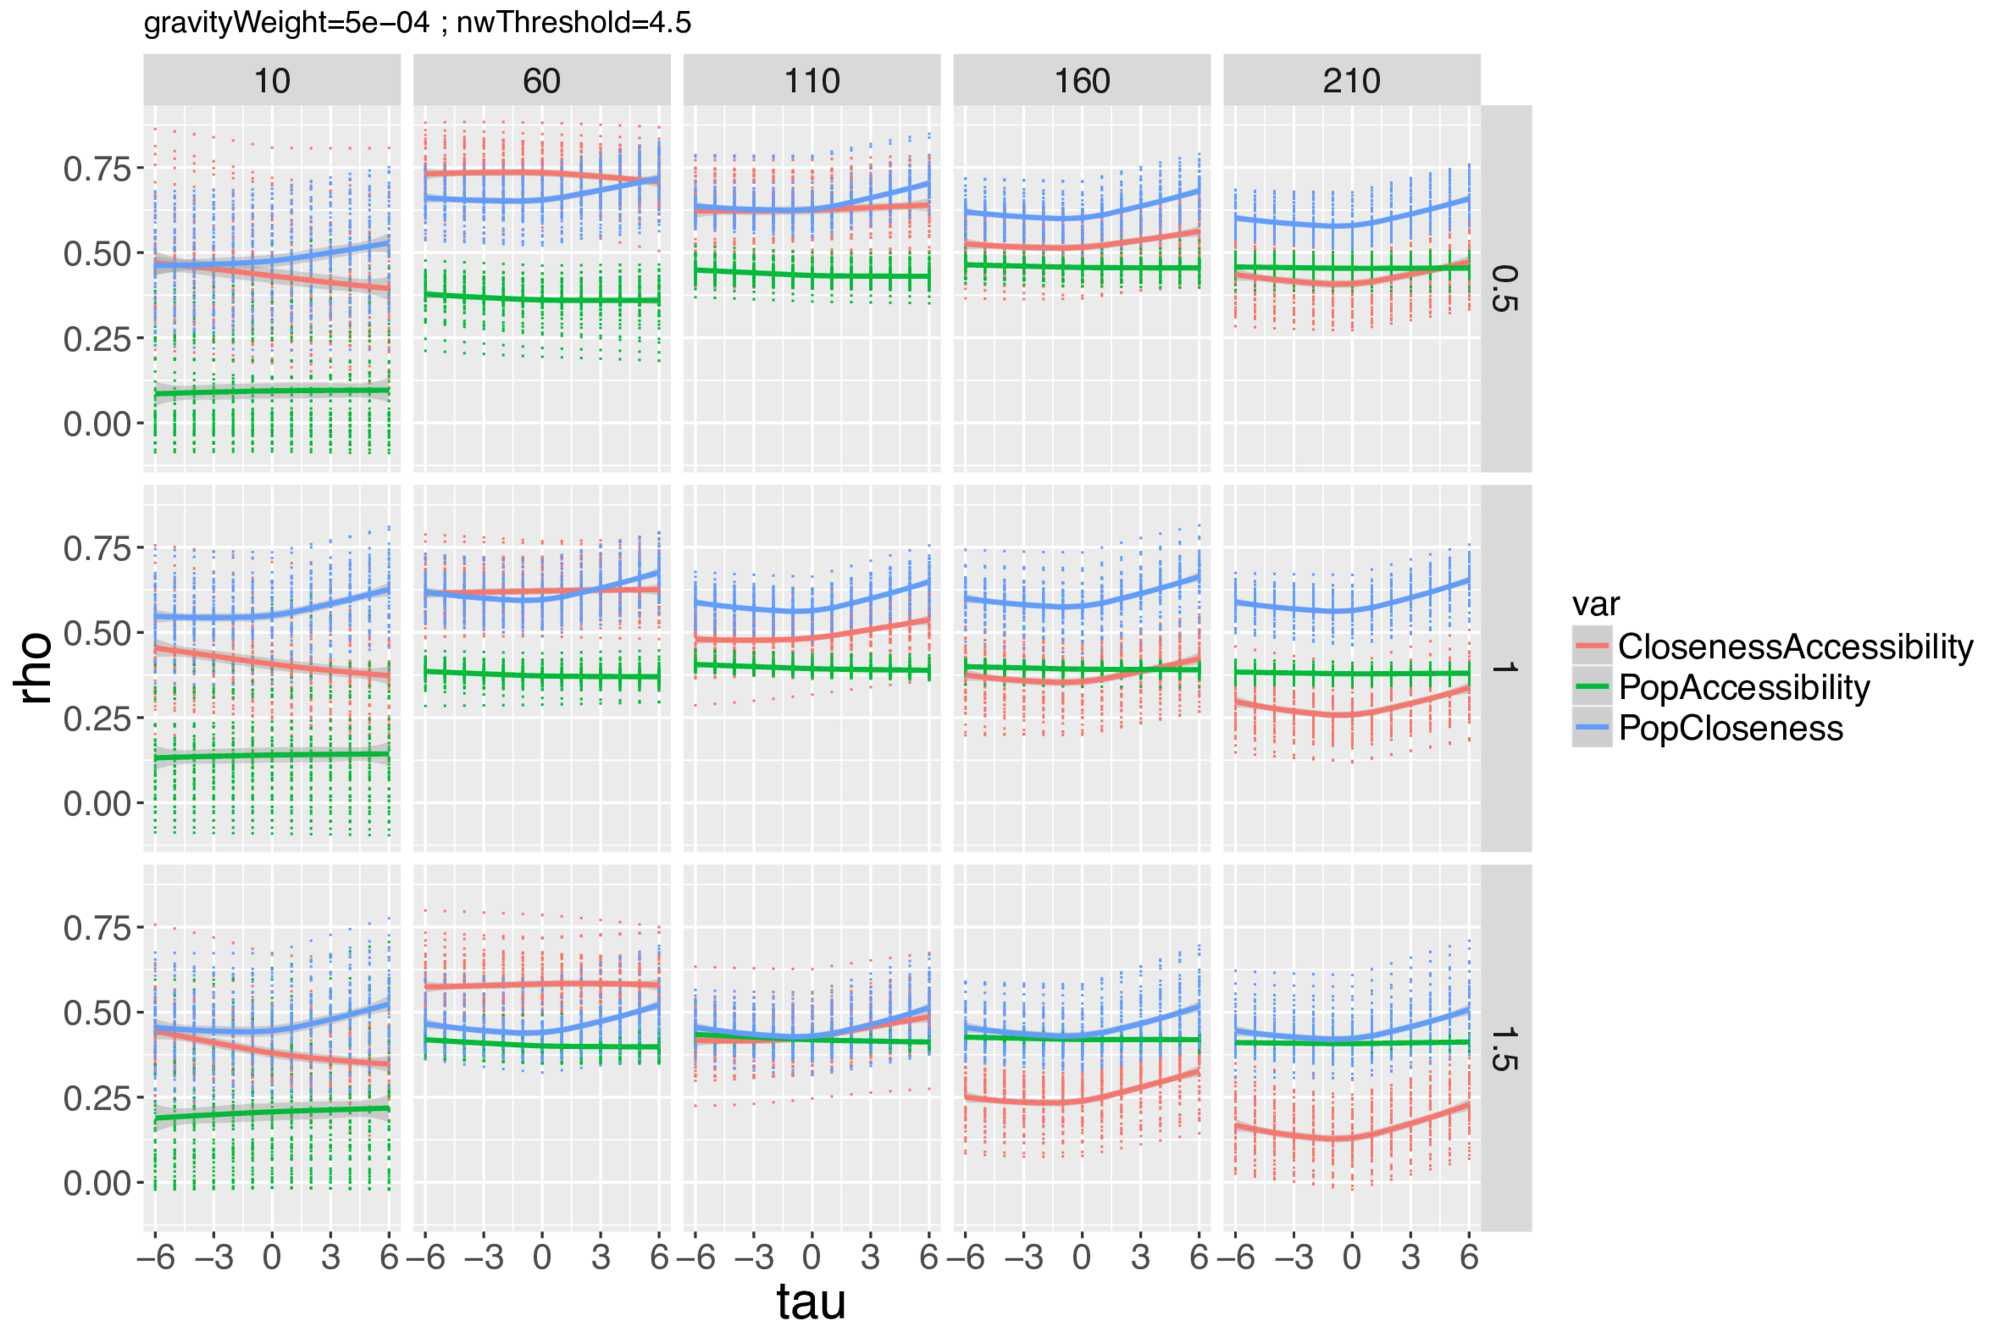
\includegraphics[width=\linewidth]{Figures/Final/A-macrocoevol-laggedcorrs.jpg}
\appcaption{\label{fig:app:macrocoevol:distcorrs}}{\textbf{Corrélations retardées.} Correlations retardées $\rho_{\tau}$ en fonction du retard $\tau$, de manière similaire pour $d_G$ variable (colonnes) et $\gamma_G$ variable (lignes), à $w_G = 5e-4$ et $\phi_0 = 4.5$.
\label{fig:app:macrocoevol:laggedcorrs}}
\end{figure}
%%%%%%%%%%%%%








%%%%%%%%%%%%%%%%%%%
\subsection{Real data}{Données réelles}





%%%%%%%%%%%%%%%%%%%
\begin{figure}
%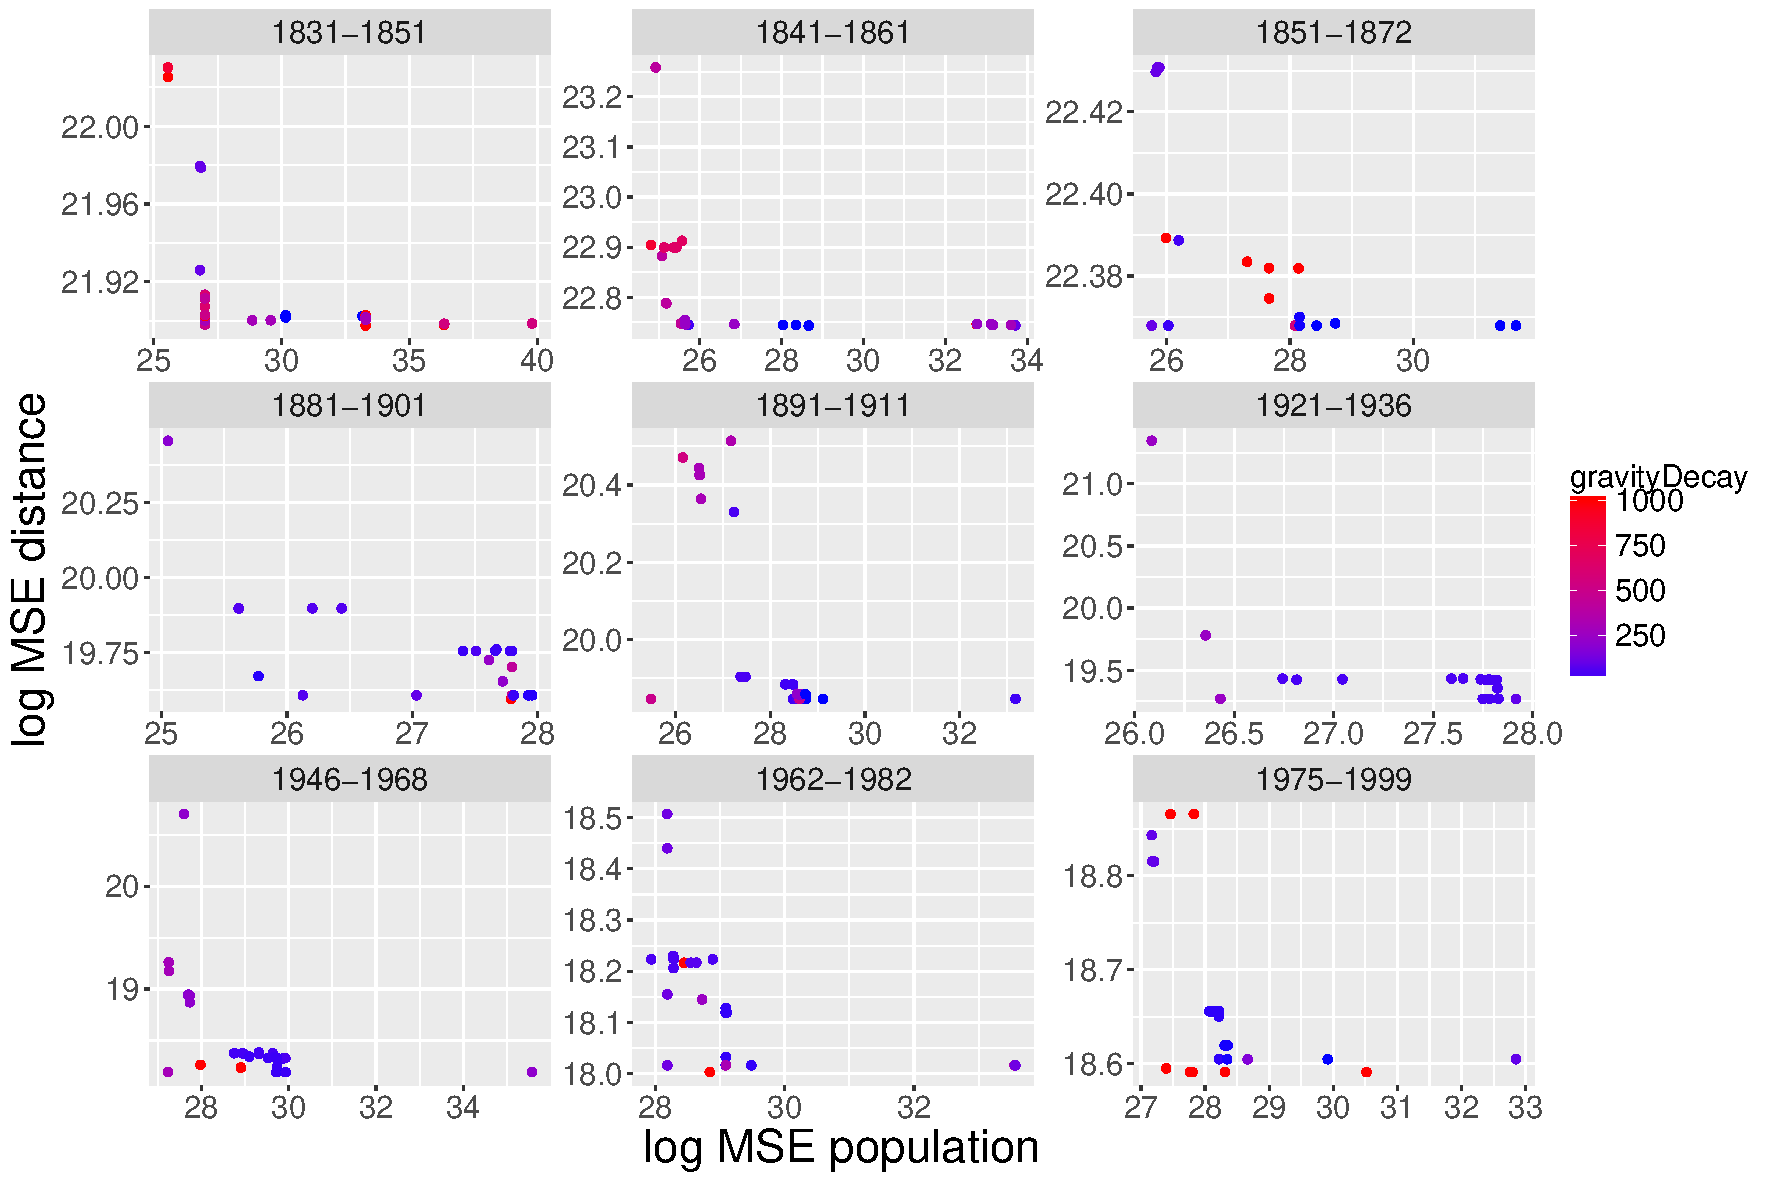
\includegraphics[width=0.9\linewidth]{Figures/MacroCoEvol/pareto_gravityDecay}
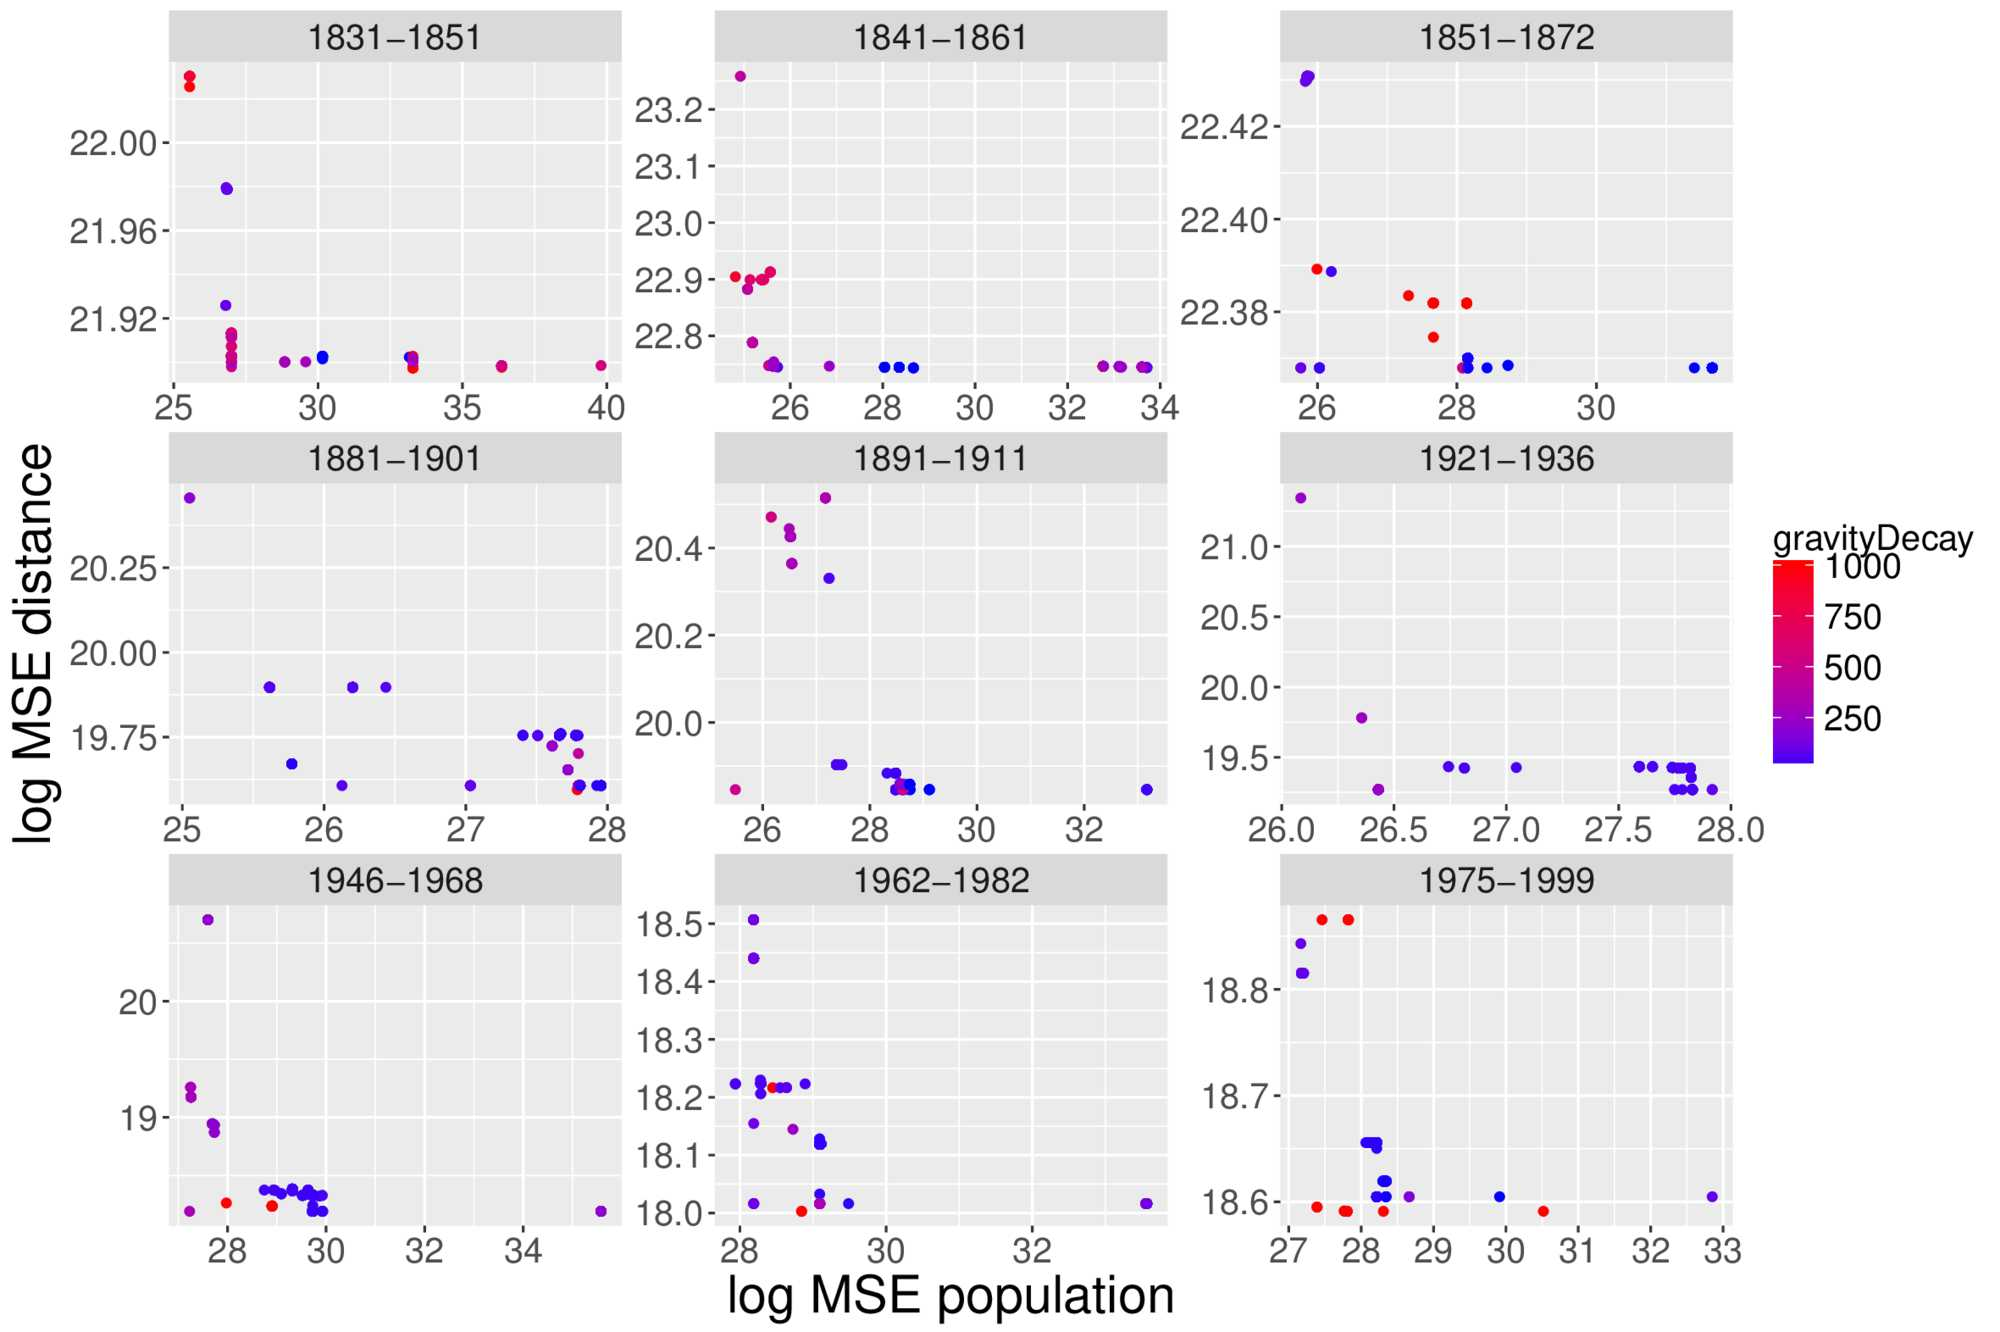
\includegraphics[width=\linewidth]{Figures/Final/A-macrocoevol-pareto.jpg}
\appcaption{\label{fig:macrocoevol:pareto}}{\textbf{Fronts de Pareto pour la calibration bi-objectif population et distance.} Les fronts sont donnés pour chaque période de calibration, et colorés en fonction de $d_G$ (Bas).\label{fig:app:macrocoevol:pareto}}
\end{figure}
%%%%%%%%%%%%%%%%%%%








